\documentclass[a4paper]{article}
\usepackage{amsmath}
\usepackage{amssymb}
\usepackage{geometry}
\usepackage{enumerate}
\usepackage{natbib}
\usepackage{float}%稳定图片位置
\usepackage{graphicx,subfig}%画图
\usepackage{caption}
\usepackage[english]{babel}
\usepackage{indentfirst}%缩进
\usepackage{enumerate}%加序号
\usepackage{multirow}%合并行
\usepackage{hyperref}
\newcommand{\reals}{{\mathbb{R}}}
\hypersetup{hypertex=true, colorlinks=true, linkcolor=black, anchorcolor=black, citecolor=black}
\title{\Large \textbf{VG441 Problem Set 1}\\
\author{\textbf{Pan, Chongdan ID:516370910121}\\
}
}
\begin{document}
\maketitle
\begin{center}
    \textbf{\Large{THE UM-SJTU JI HONOR CODE}}
\end{center}

\noindent\textbf{I accept the letter and spirit of the honor code:\\\\
I have neither given nor received unauthorized aid on this examination, nor have
I concealed any violations of the Honor Code by myself or others.\\\\Signature:}

\section{Problem 1}
    \begin{enumerate}[(a)]
        \item   \quad\\
            \begin{figure}[H]
                \centering
                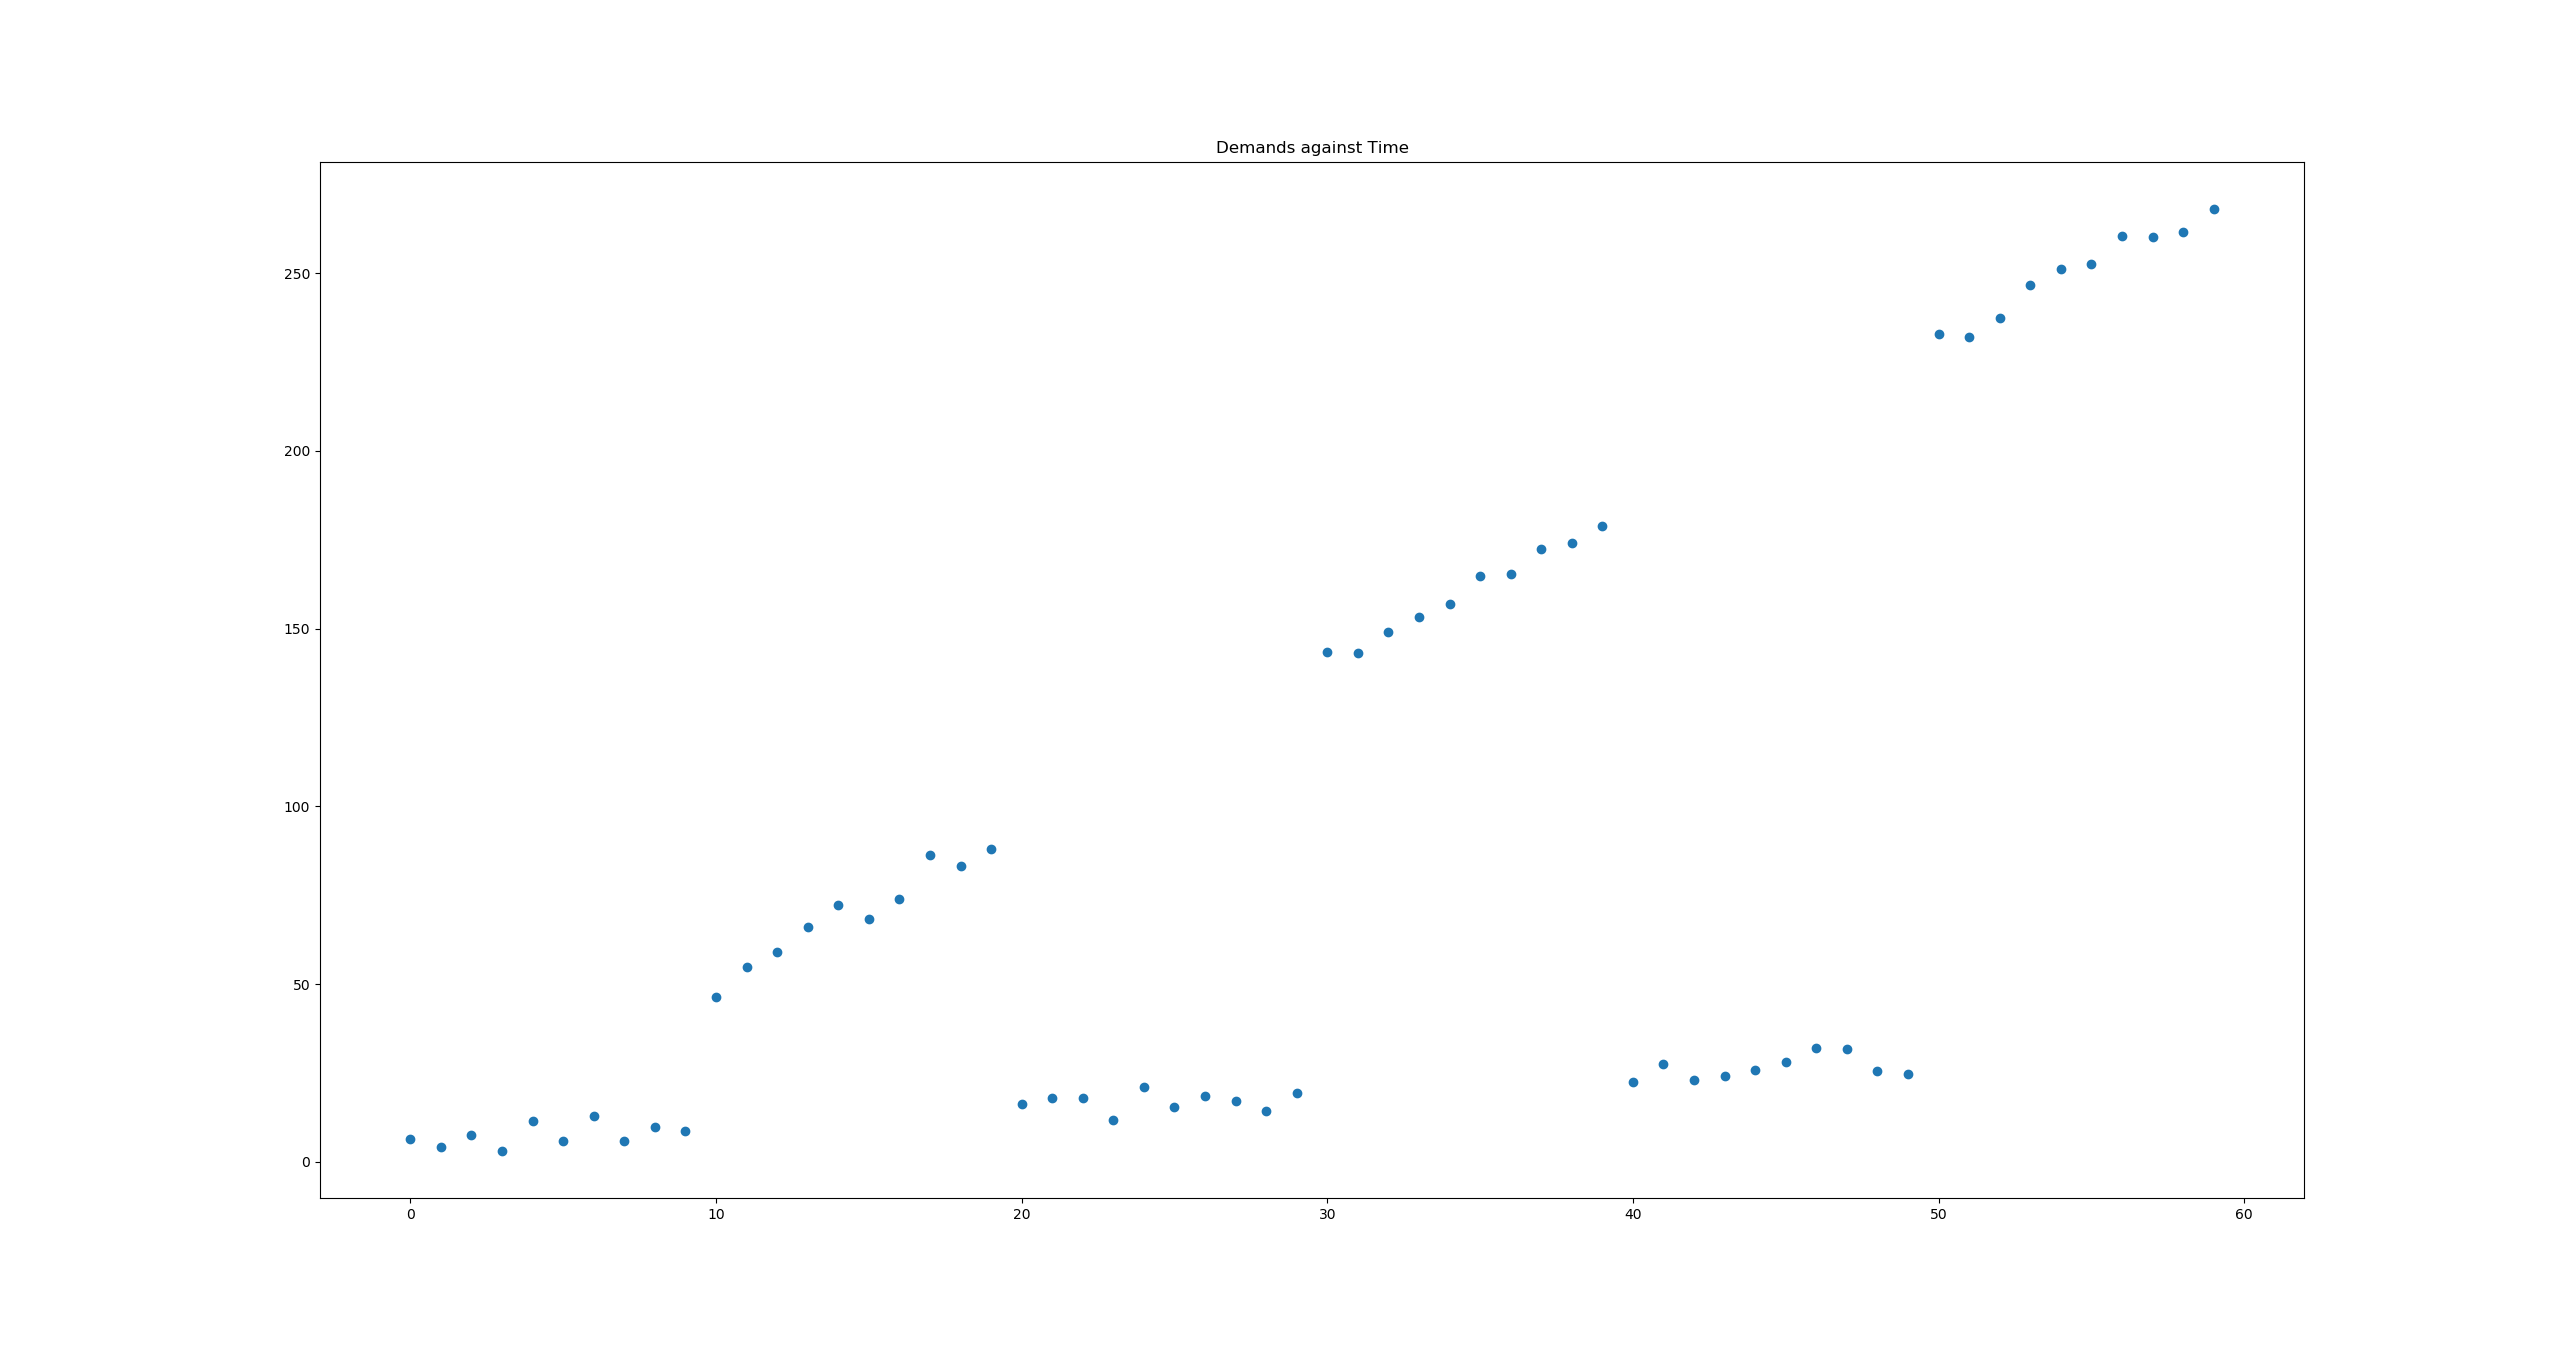
\includegraphics[scale=0.25]{P1a.png}
                \caption{demands against time}
            \end{figure}
        \item   \quad\\
        \begin{figure}[H]
            \centering
            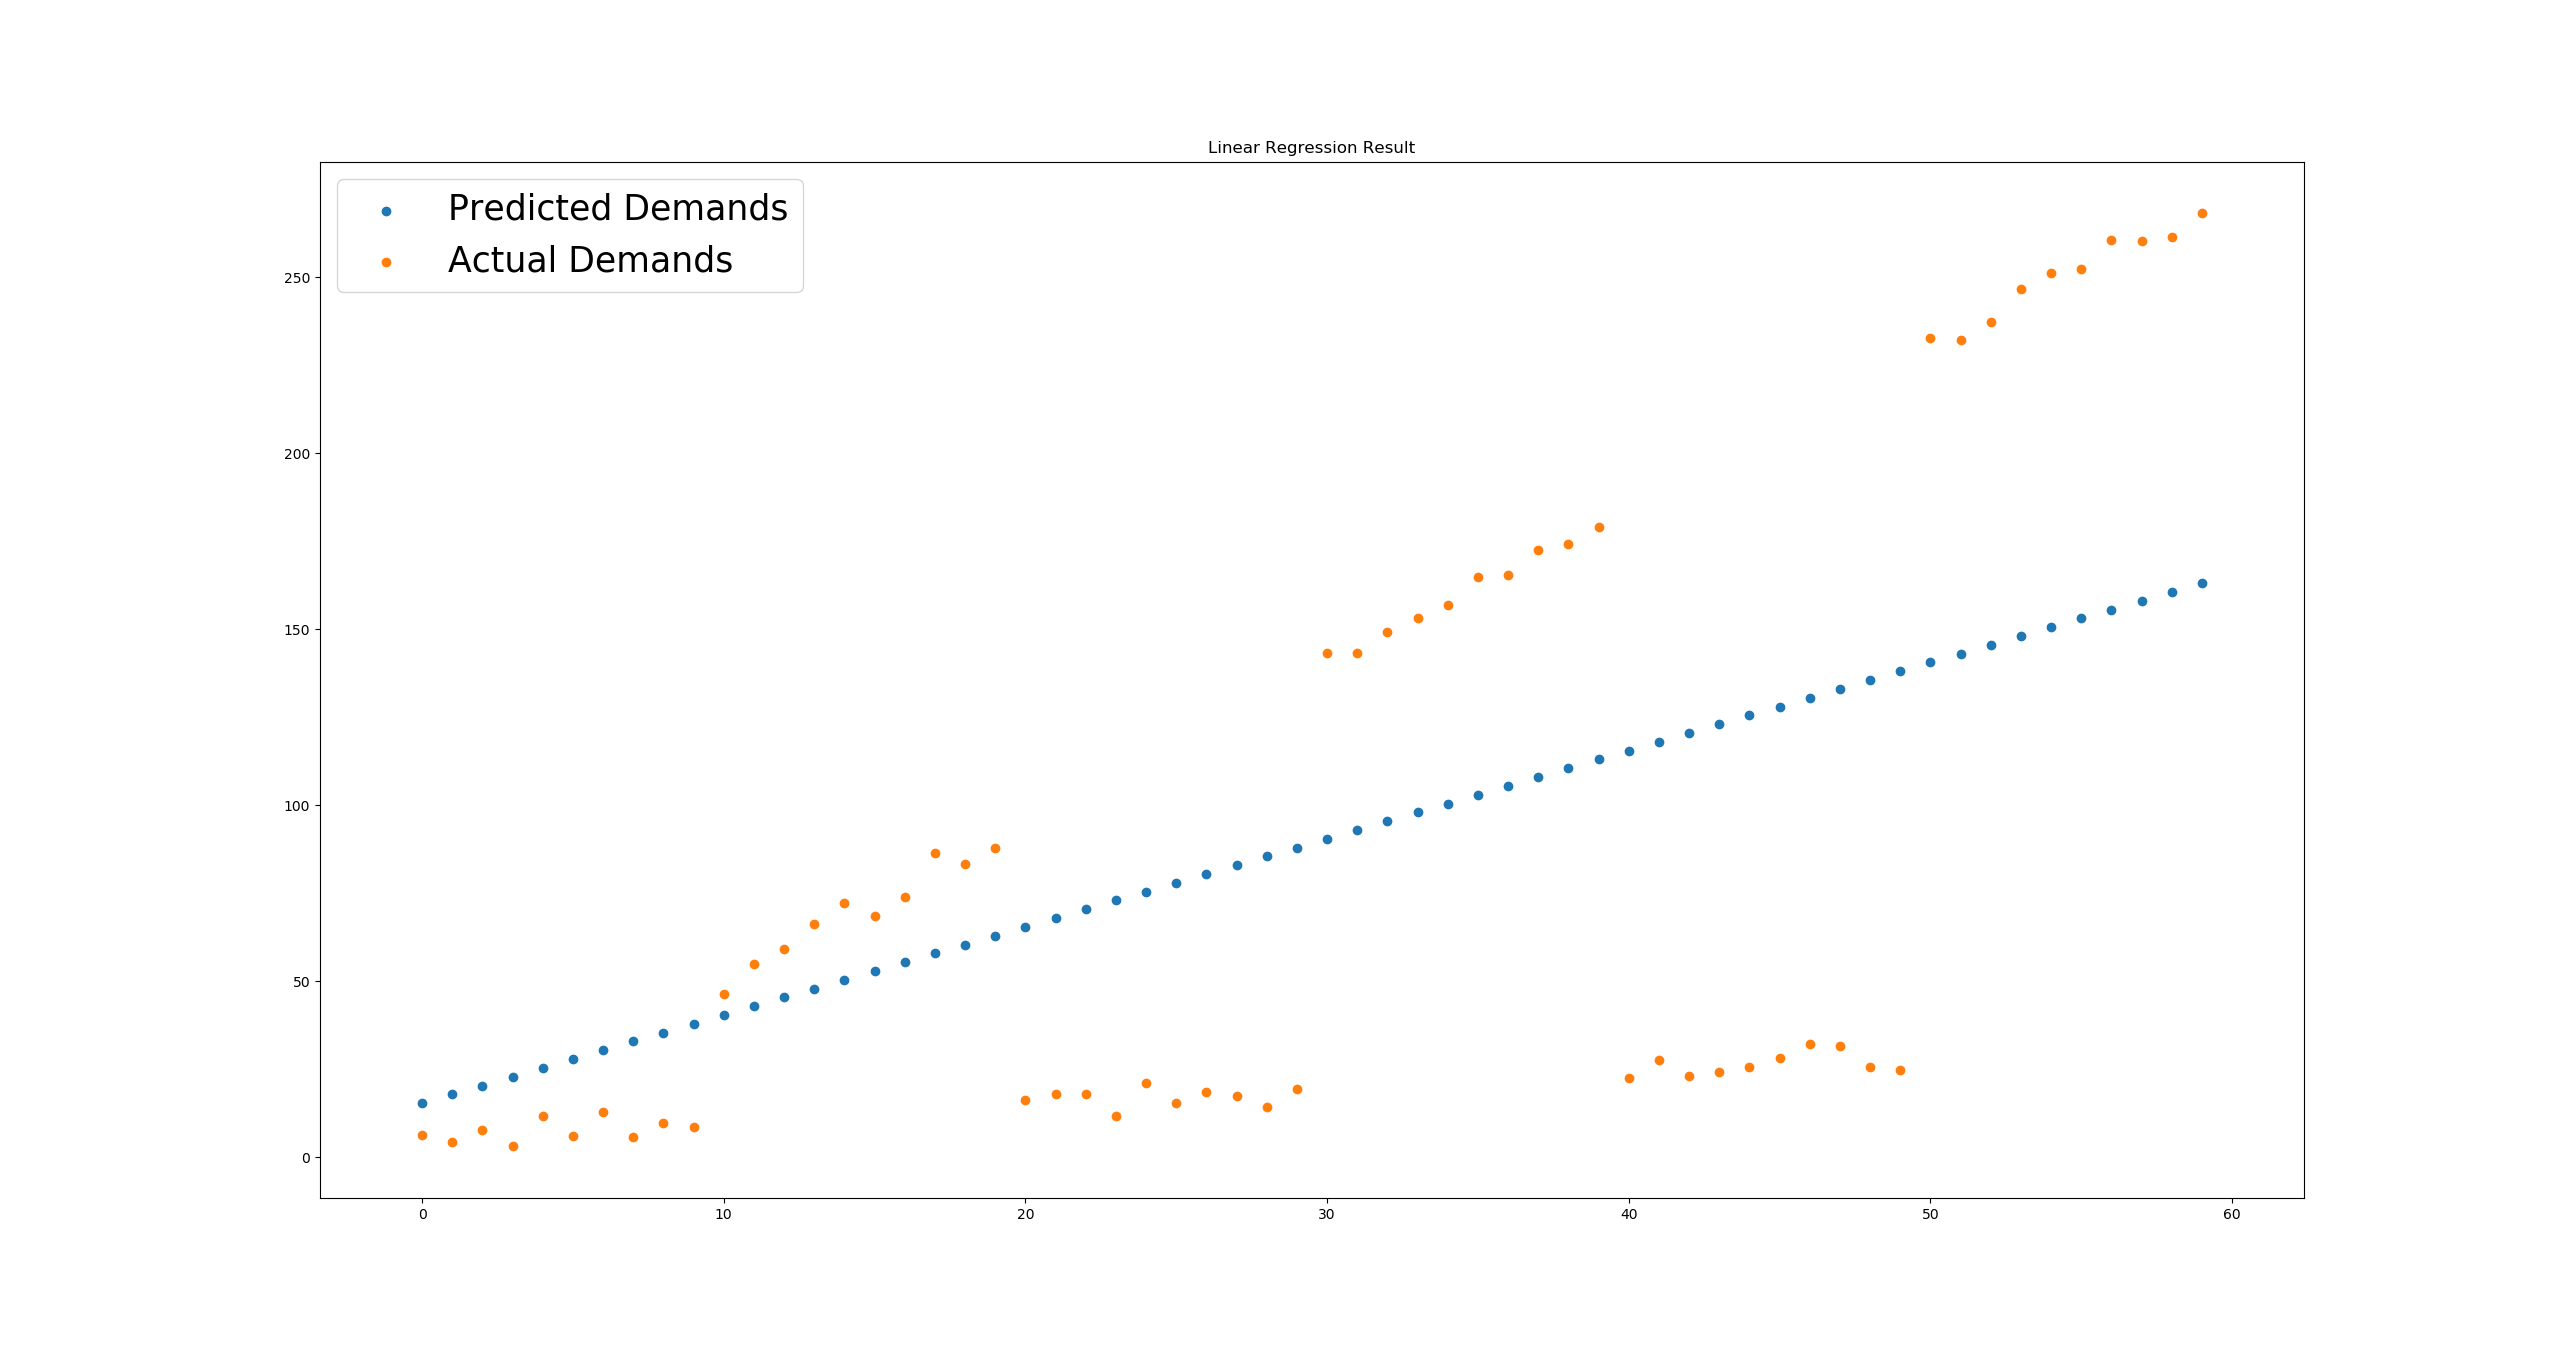
\includegraphics[scale=0.25]{P1b.png}
            \caption{Linear Regression Result}
        \end{figure}
        \item   \quad\\
        \begin{figure}[H]
            \centering
            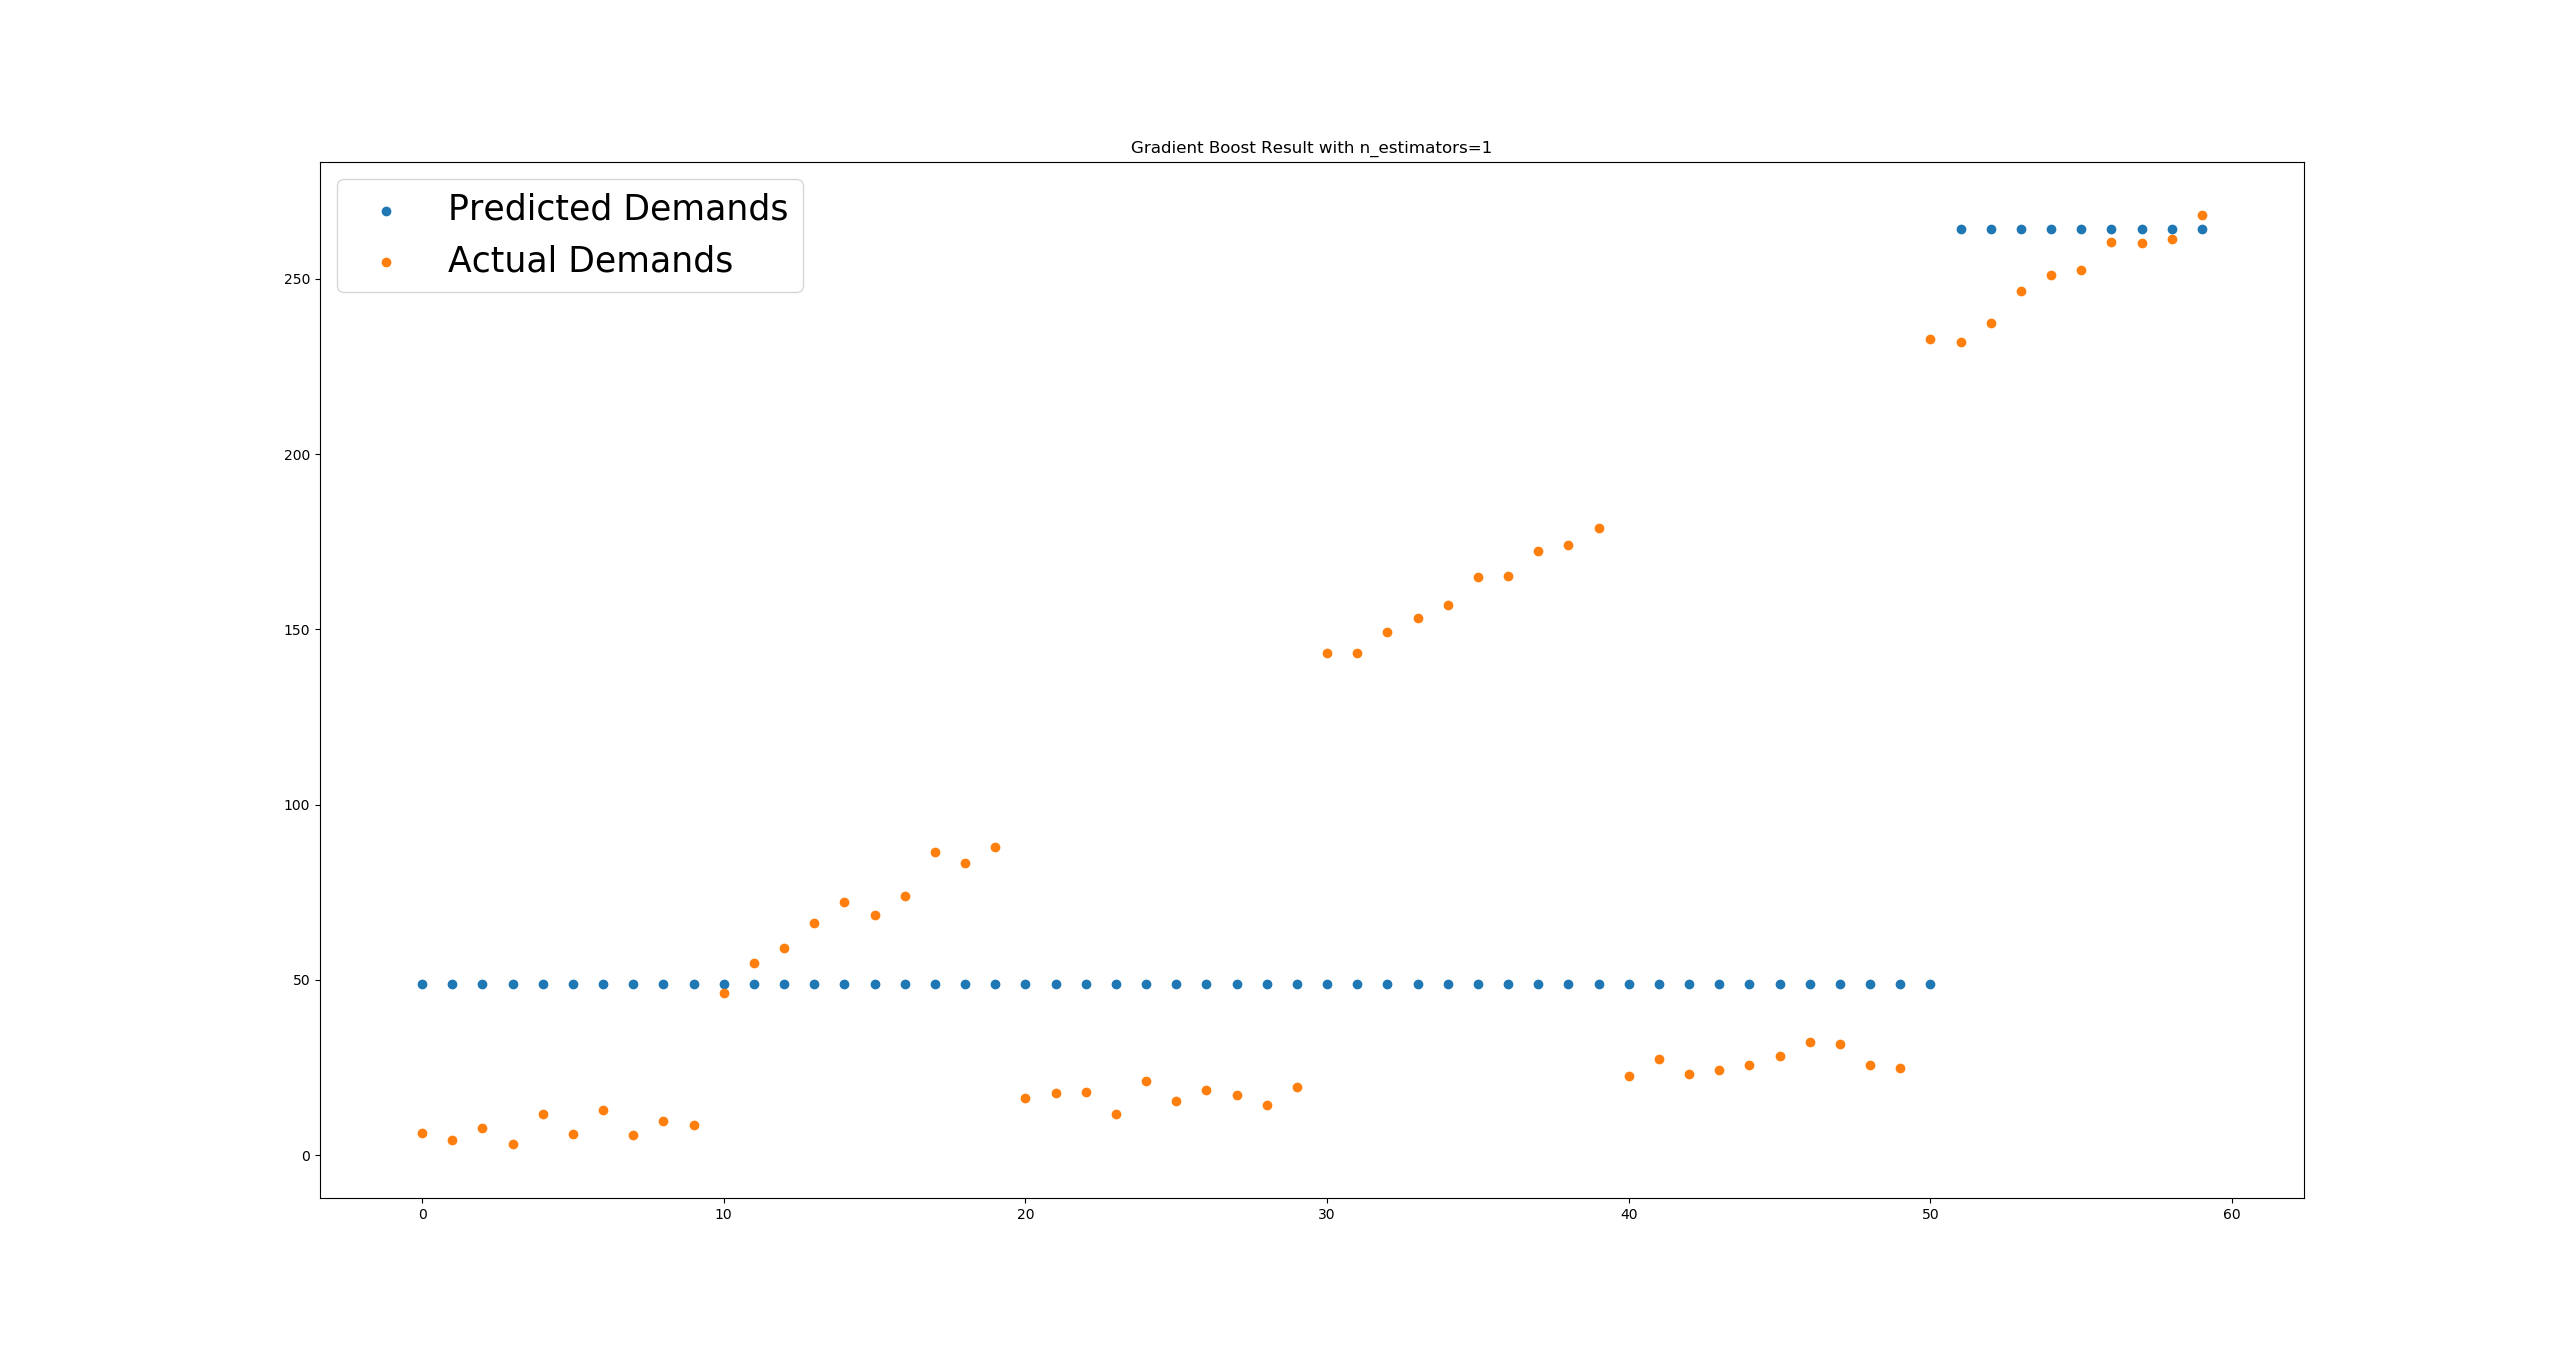
\includegraphics[scale=0.25]{P1c1.png}
            \caption{Gradient Boost Result with n\_estimators=1}
        \end{figure}
        \begin{figure}[H]
            \centering
            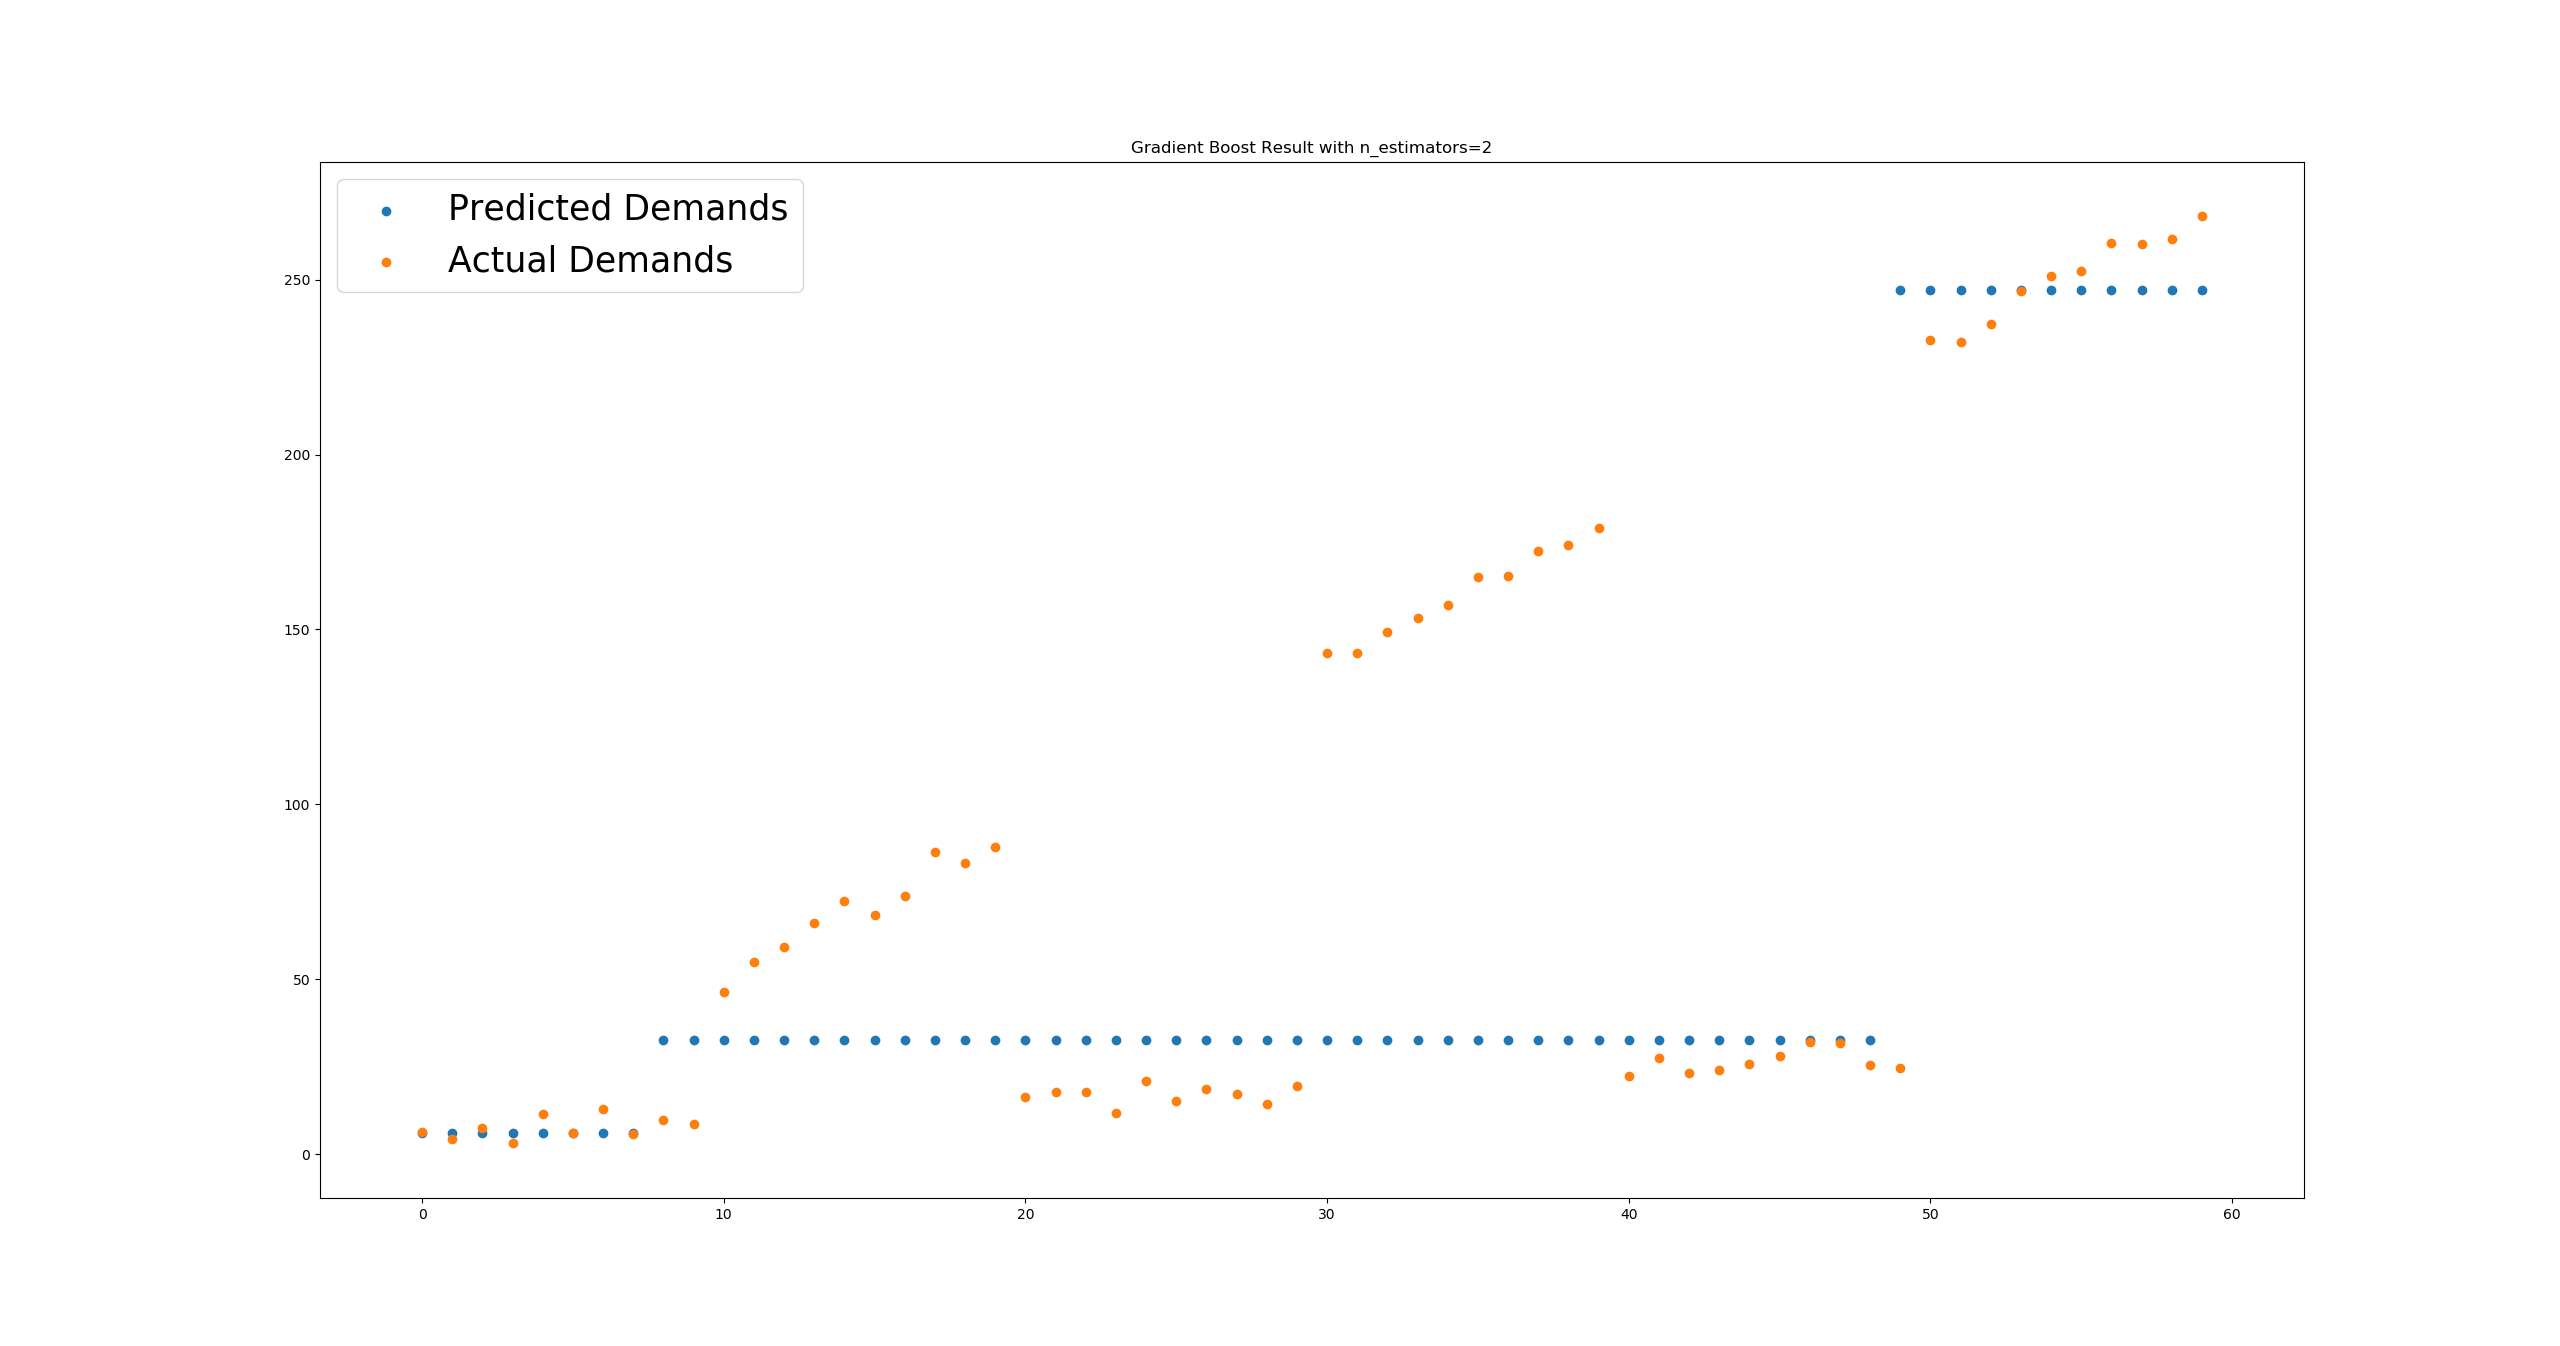
\includegraphics[scale=0.25]{P1c2.png}
            \caption{Gradient Boost Result with n\_estimators=2}
        \end{figure}
        \begin{figure}[H]
            \centering
            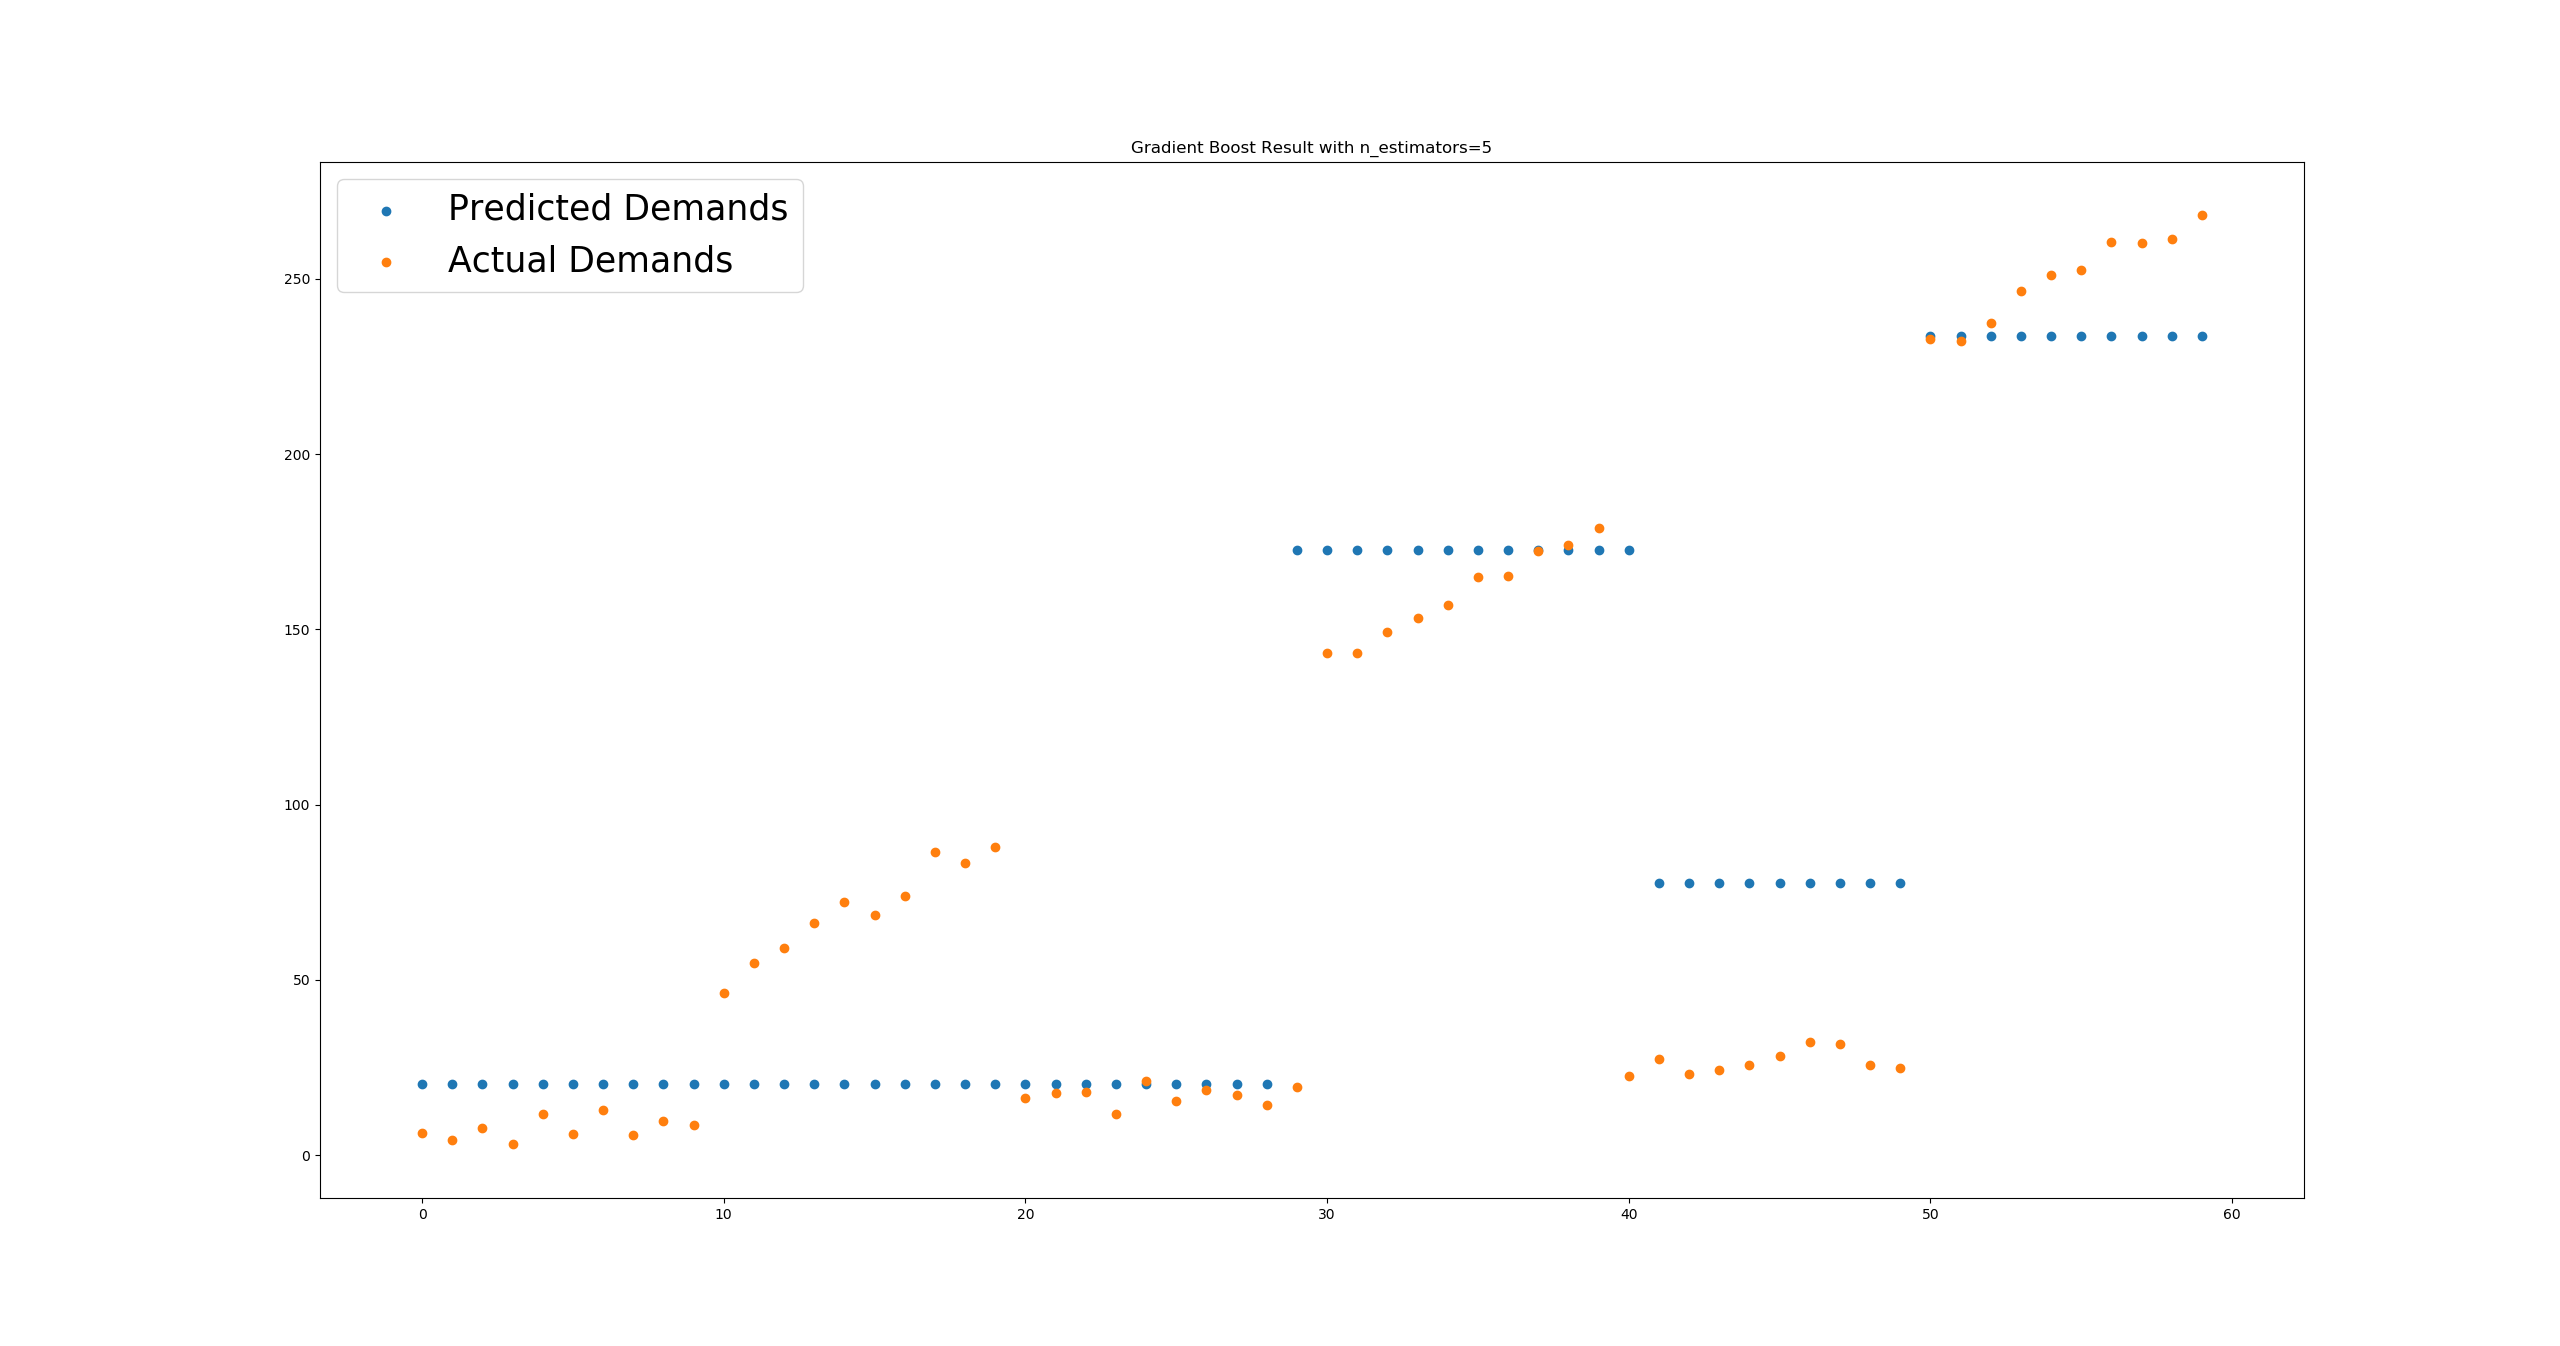
\includegraphics[scale=0.25]{P1c3.png}
            \caption{Gradient Boost Result with n\_estimators=5}
        \end{figure}
        \begin{figure}[H]
            \centering
            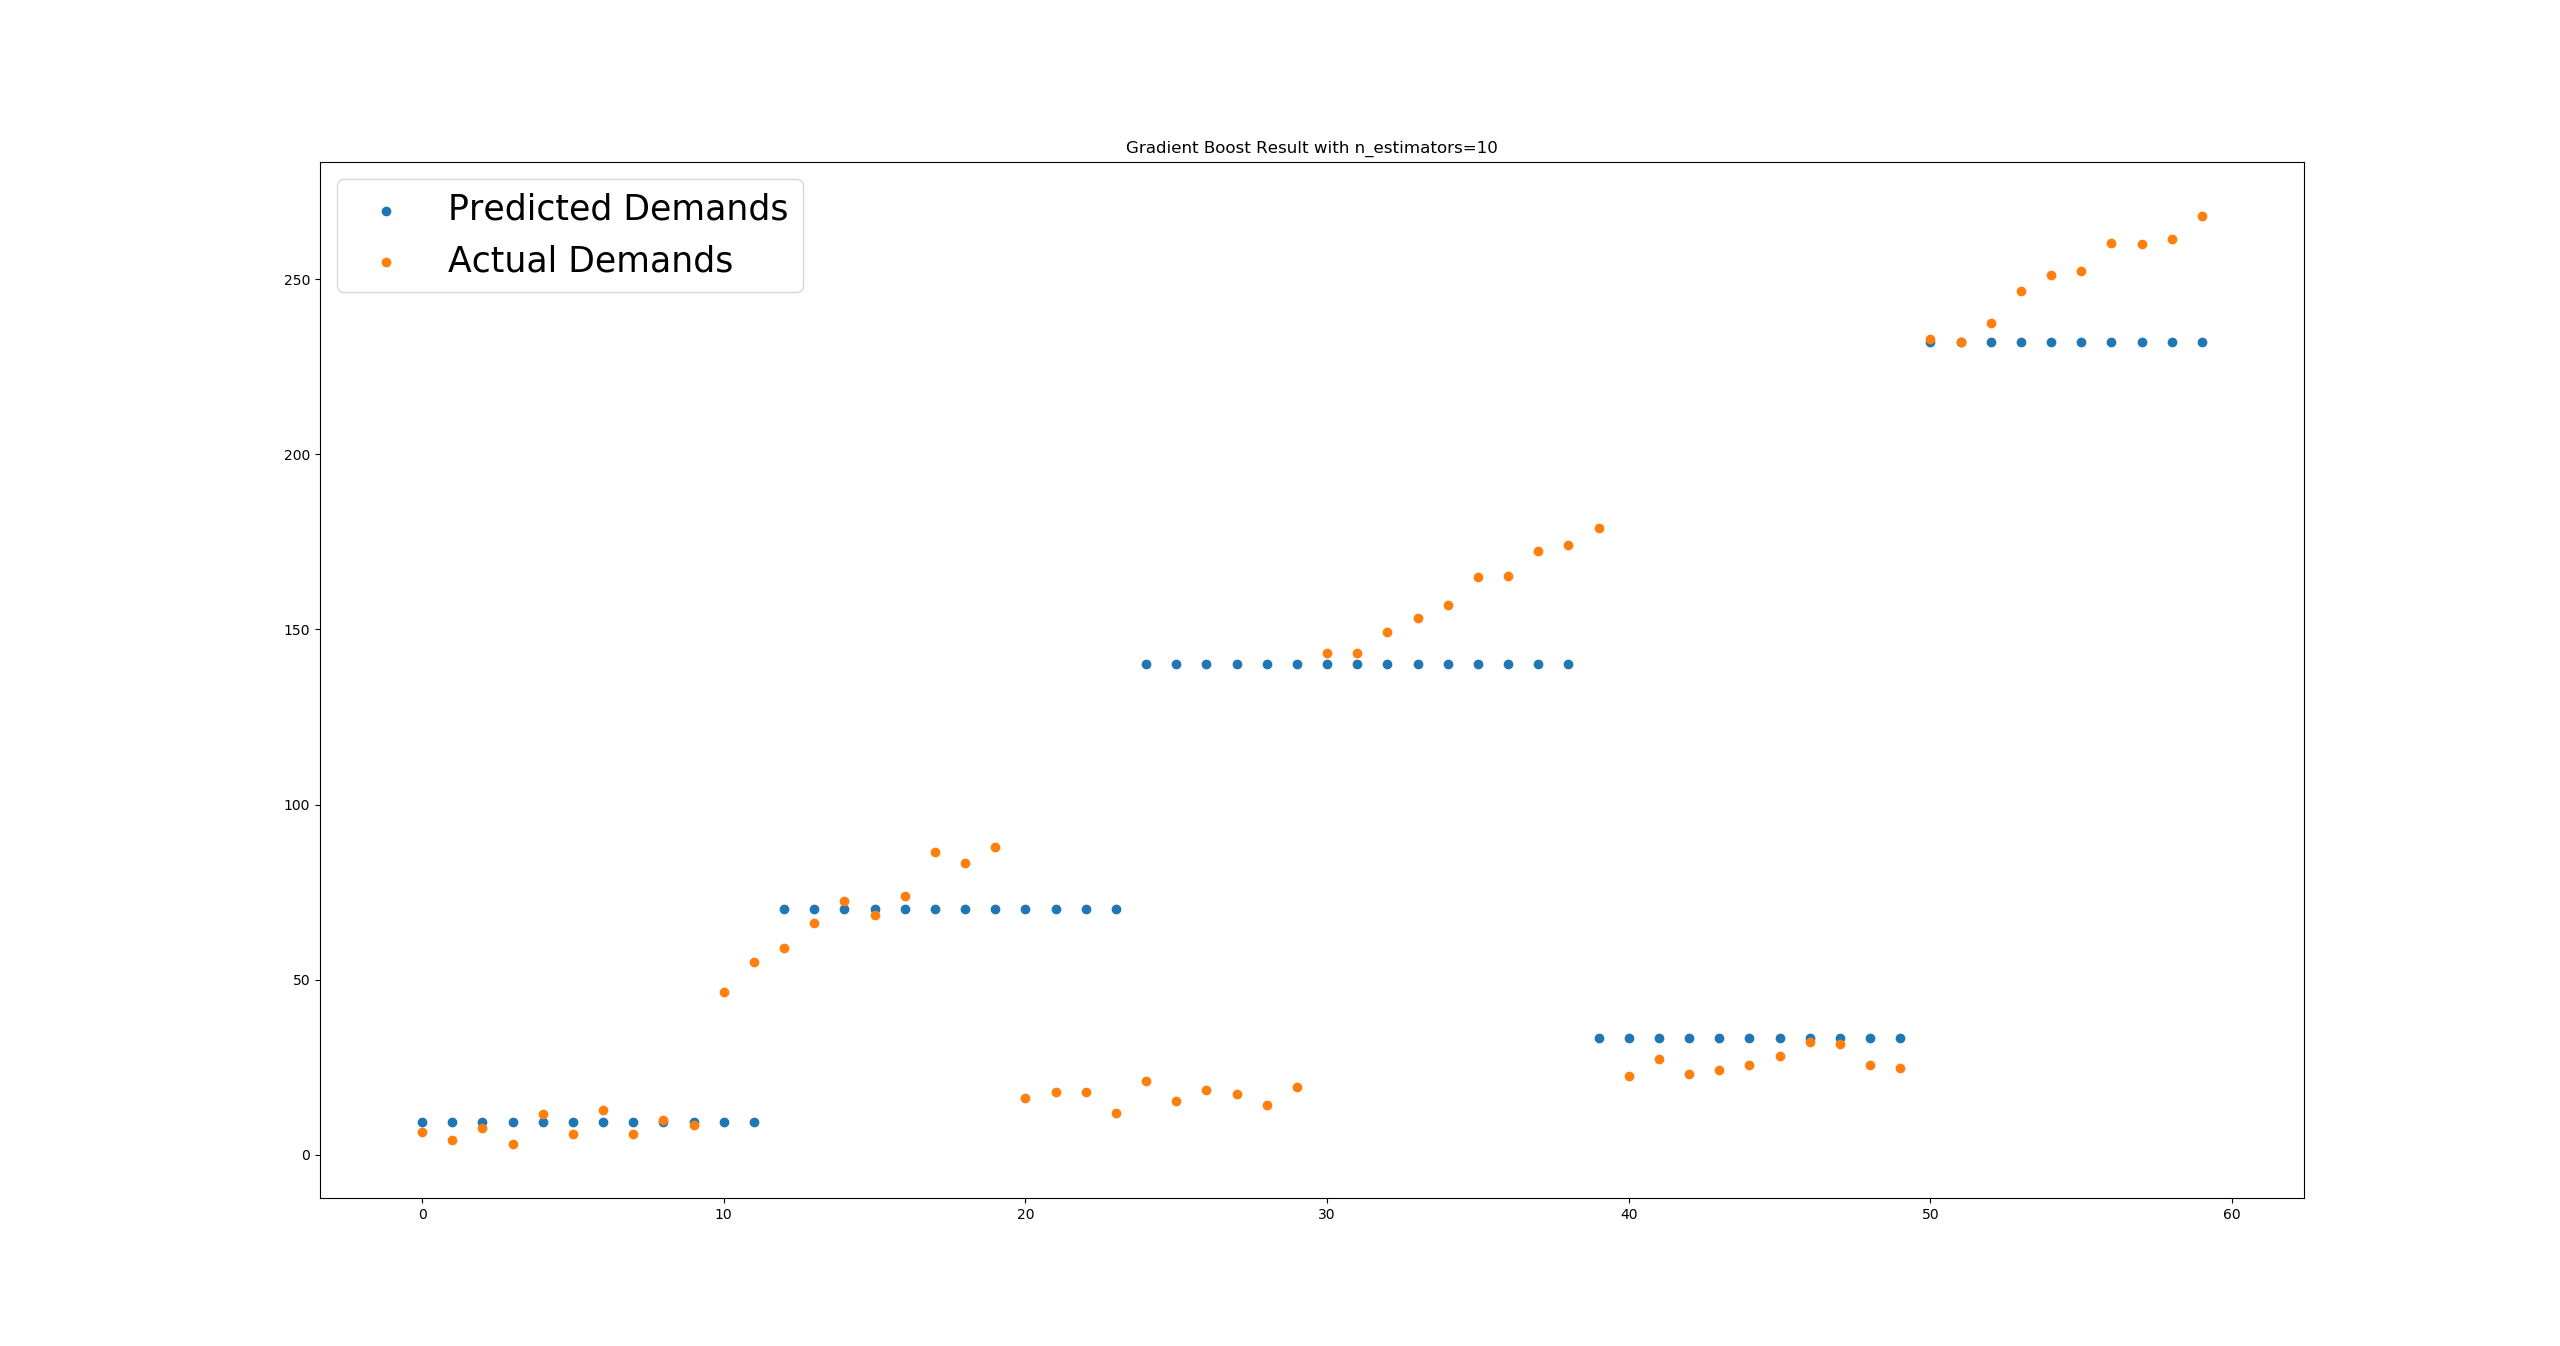
\includegraphics[scale=0.25]{P1c4.png}
            \caption{Gradient Boost Result with n\_estimators=10}
        \end{figure}
        \begin{figure}[H]
            \centering
            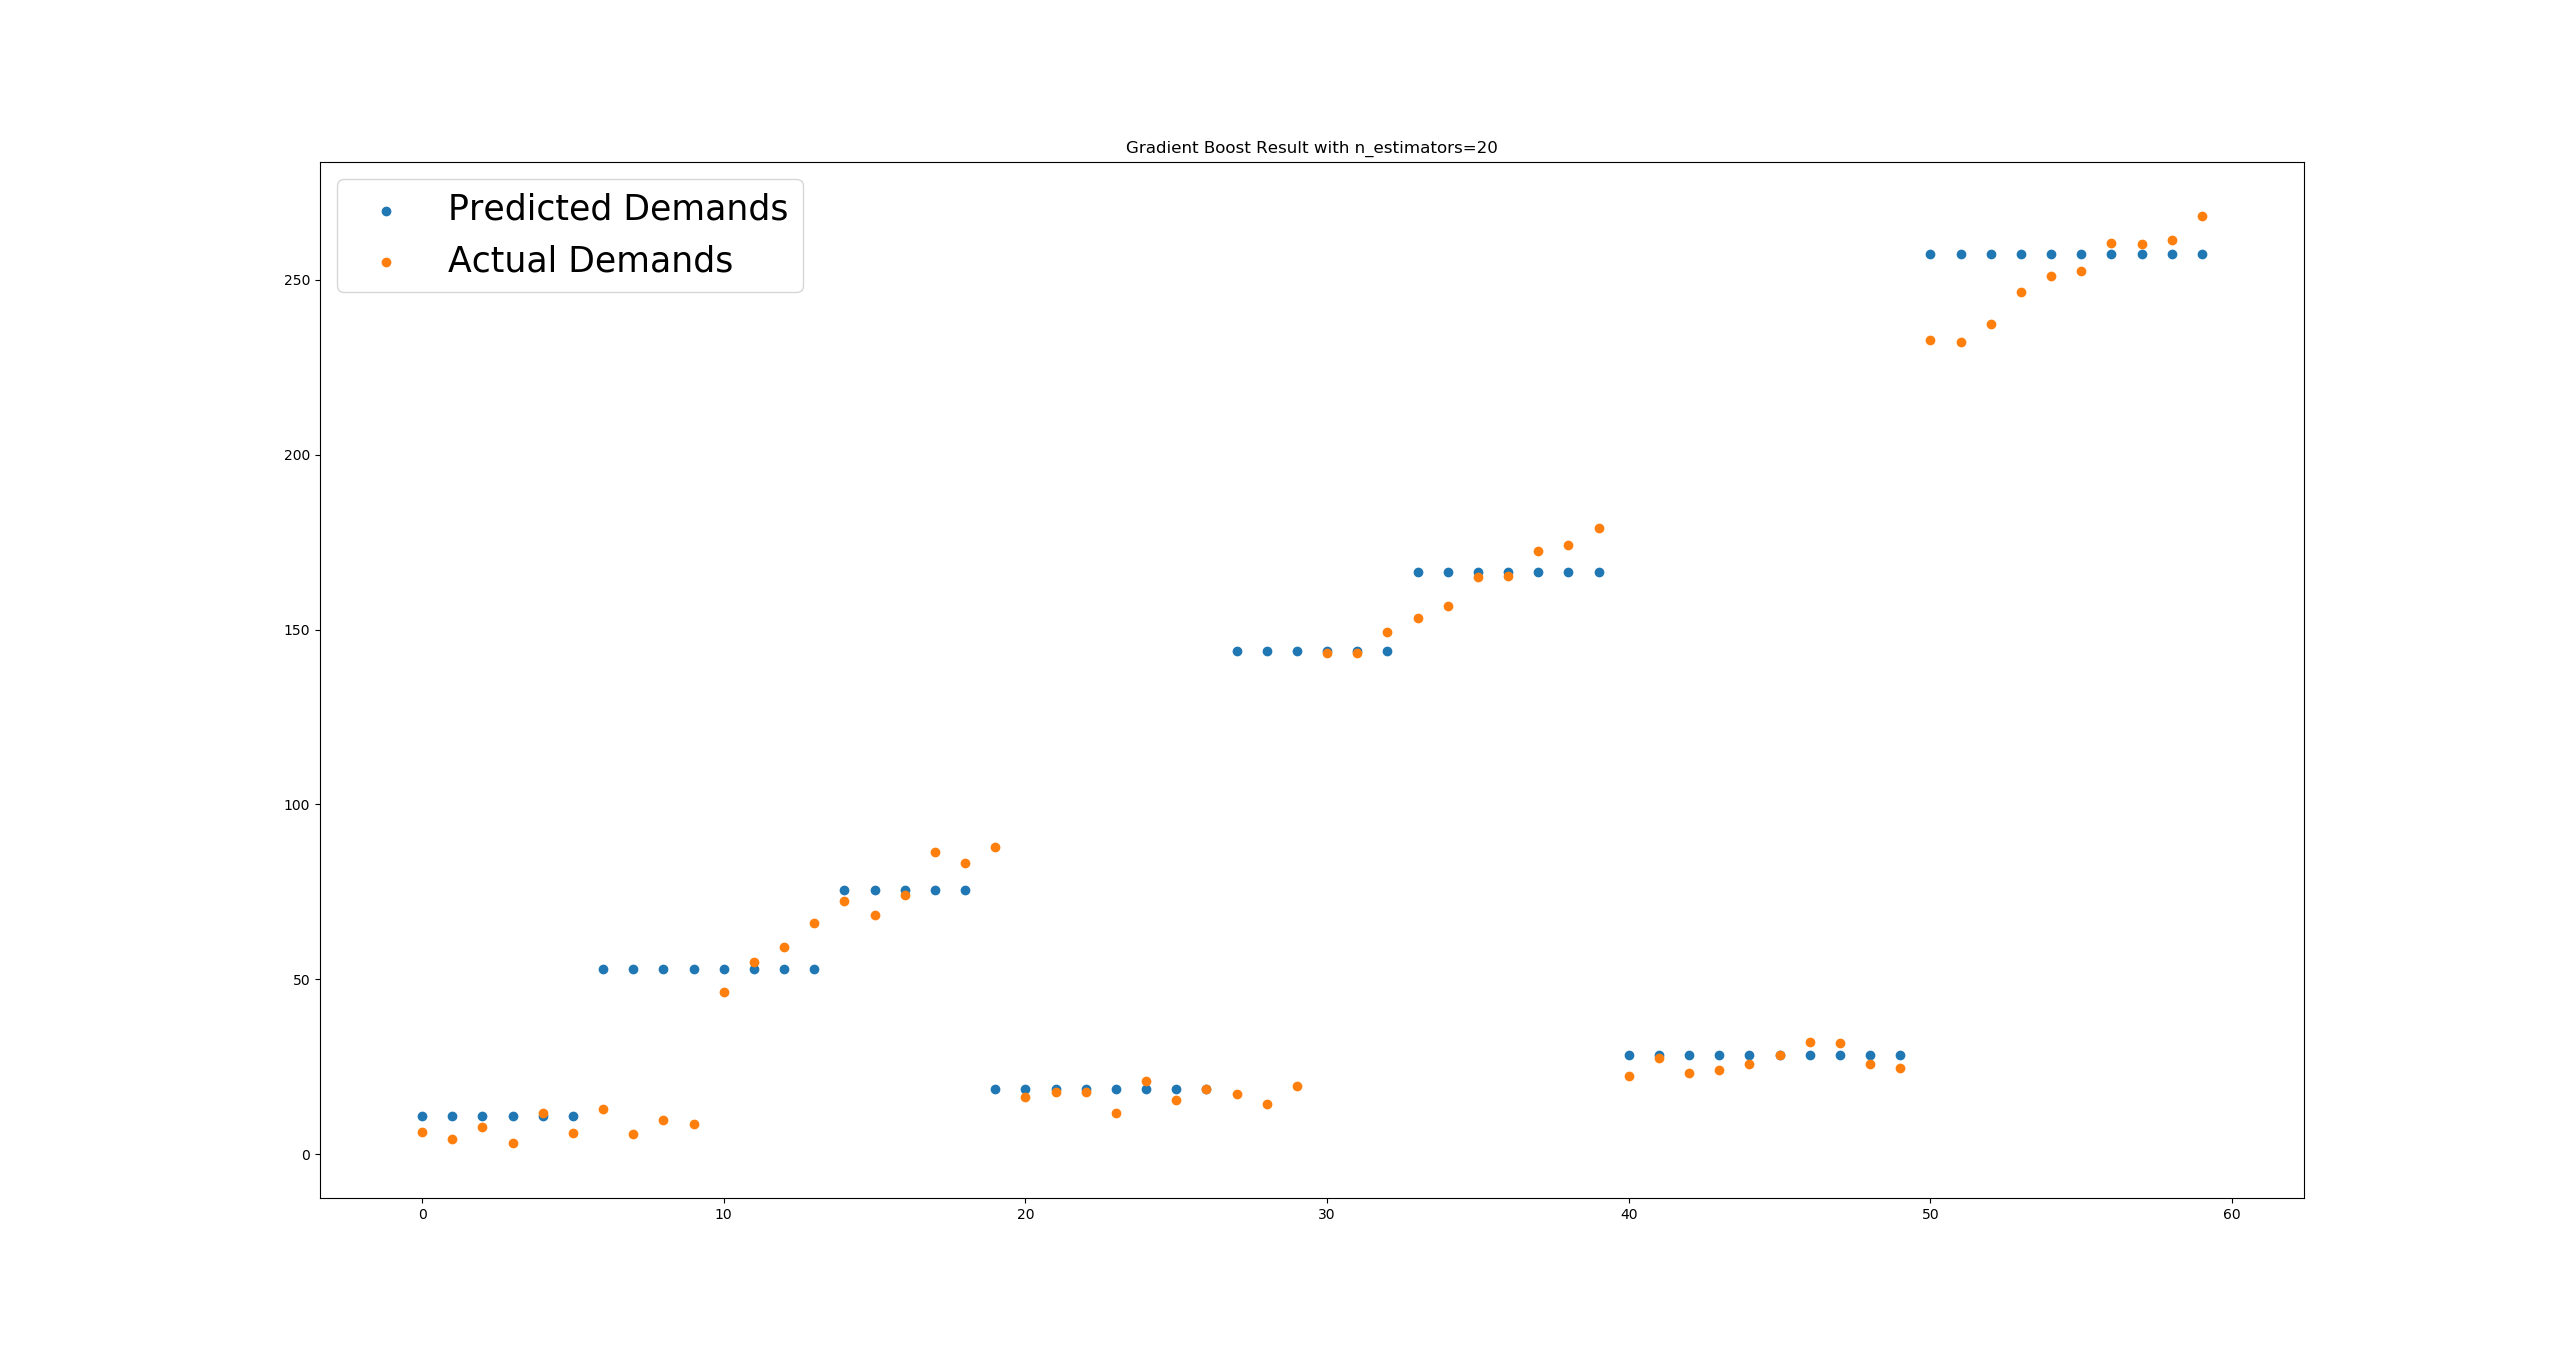
\includegraphics[scale=0.25]{P1c5.png}
            \caption{Gradient Boost Result with n\_estimators=20}
        \end{figure}
        \begin{figure}[H]
            \centering
            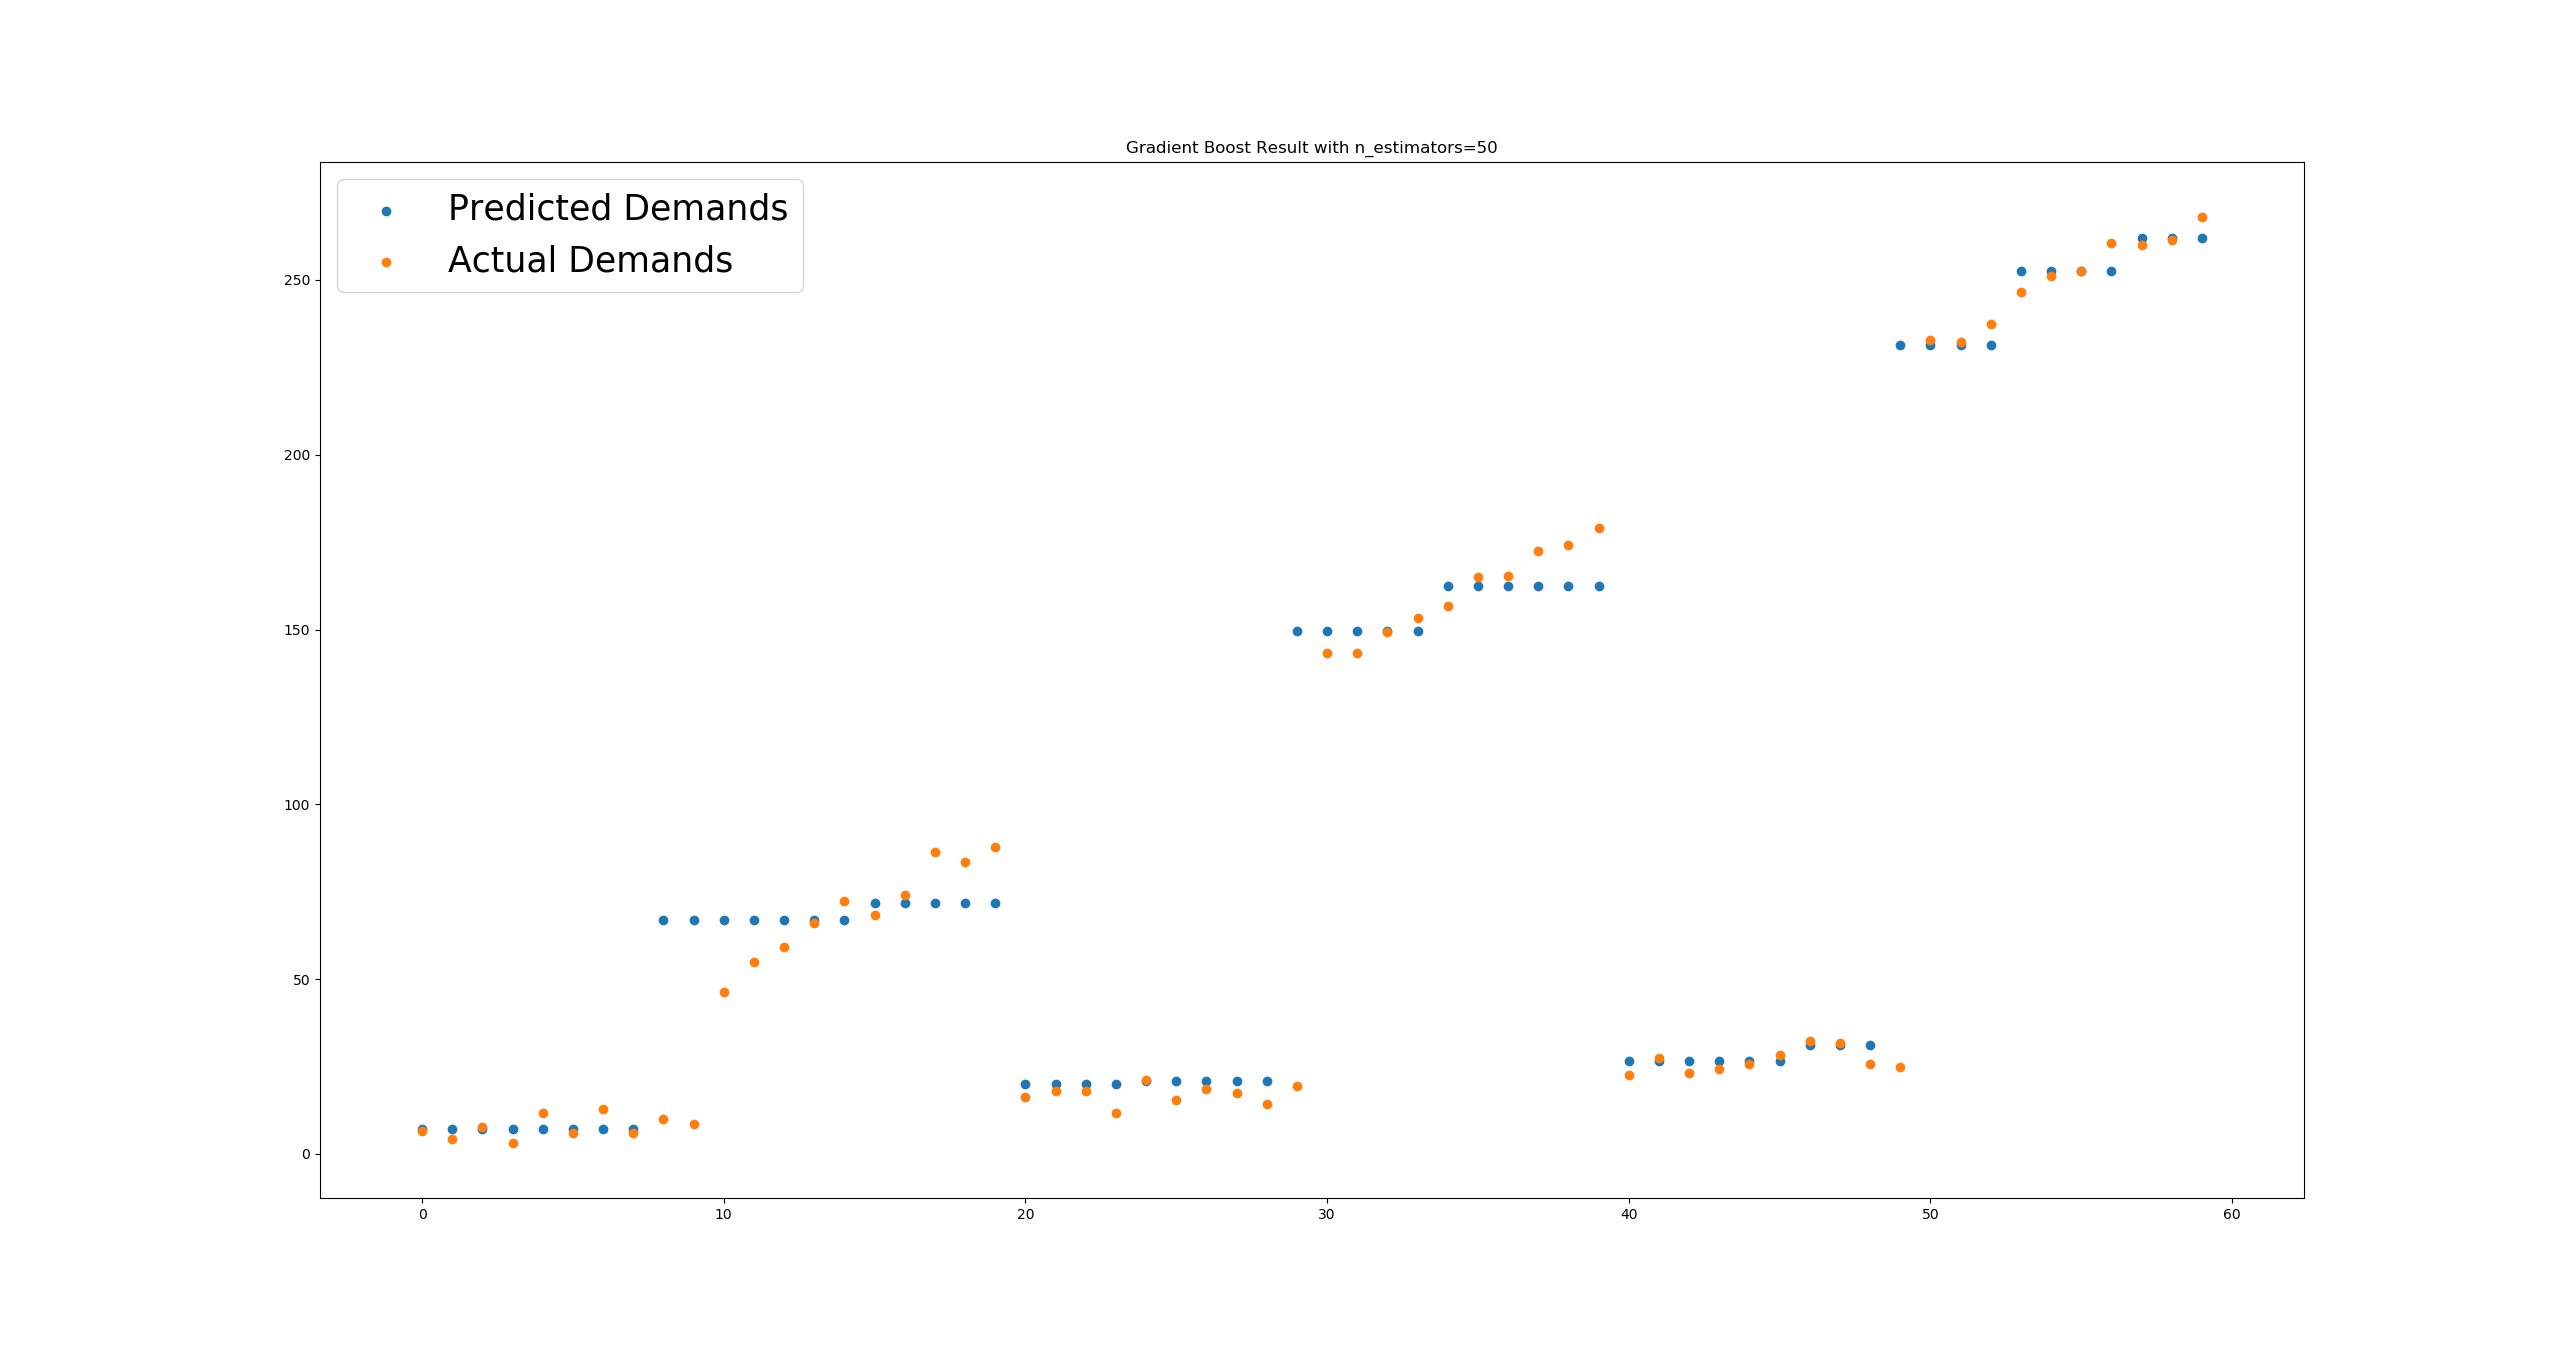
\includegraphics[scale=0.25]{P1c6.png}
            \caption{Gradient Boost Result with n\_estimators=50}
        \end{figure}
    \end{enumerate}
\section{Problem 2}
    \begin{enumerate}[(a)]
        \item $K=\$50$ per order, $h=\$\frac{50}{3}$ per unit per month, $\lambda=50$ units per month
        \\\[c=\begin{cases}
            520 & Q<12\\
            510 & 12\leq Q\leq64\\
            495 & 65\leq Q\leq128\\
            485 & Q>128
        \end{cases}\]
        Since it's all unit discount model, we calculate the $Q^*$ first.
        \\$Q^*=\sqrt{\frac{2K\lambda}{h}}=\sqrt{\frac{2\times50\times50}{\frac{50}{3}}}\approx17.3$
        \\So the price should be \$510
        \\$g_0(Q_*)=510\times50+\sqrt{2\times50\times50\times\frac{50}{3}}=25788.68\$$
        \\Now we calculate the cost at breakpoints:
        \\$g_0(1)=520\times50+\frac{50\times50}{1}+\frac{50}{3}\frac{1}{2}\approx28508.33$
        \\$g_1(12)=510\times50+\frac{50\times50}{12}+\frac{50}{3}\frac{12}{2}\approx25808.33\$$
        \\$g_2(65)=495\times50+\frac{50\times50}{65}+\frac{50}{3}\frac{65}{2}\approx25330.13\$$
        \\$g_2(128)=495\times50+\frac{50\times50}{128}+\frac{50}{3}\frac{128}{2}\approx25836.2\$$
        \\$g_3(129)=485\times50+\frac{50\times50}{129}+\frac{50}{3}\frac{129}{2}\approx25334.38\$$
        \\Therefore, the optimal order is not at breakpoints, the optimal quantity is $Q=65$, which incurs a purchase cost of $495\$$ and a total monthly cost of $25330.13\$$
        \item If the offer is accepted, the monthly cost will be $50\times(520+50)=28500\$$, which is larger than our optimal strategy, hence Zeus should not accept the offer.
    \end{enumerate}
\section{Problem 3}
    \begin{enumerate}[(a)]
        \item $K=\$1000,h=\$1.2$
        \\$\theta_8=0$
        \\\\$\theta_7=K+\theta_8=1000$
        \\\\$\theta_6=K+\min\{\theta_7,hd_7\}$
        \\$=1000+\min\{1000,1.2\times290\}$
        \\$=1000+\min\{1000,348\}=1348$
        \\\\$\theta_5=K+\min\{\theta_6,hd_6+\theta_7,h(d_6+2\times d_7)+\theta_8\}$
        \\$=1000+\min\{1348,1.2\times 210+1000,1.2\times(210+2\times290)\}$
        \\$=1000+\min\{1348,1252,948\}=1948$
        \\\\$\theta_4=K+\min\{\theta_5,hd_5+\theta_6,h(d_5+2\times d_6)+\theta_7,h(d_5+2\times d_6+3\times d_7)+\theta_8\}$
        \\$=1000+\min\{1948,1.2\times170+1348,1.2\times(170+2\times210)+1000,1.2\times(170+2\times210+3\times290)\}$
        \\$=\min\{2948,2552,2708,2752\}=2552$
        \\\\$\theta_3=K+\min\{\theta_4,hd_4+\theta_5,h(d_4+2\times d_5)+\theta_6,h(d_4+2\times d_5+3\times d_6)+\theta_7,h(d_4+2\times d_5+3\times d_6+4\times d_7)+\theta_8\}$
        \\$=1000+\min\{2552,1.2\times90+1948,1.2\times(90+2\times170)+1348,1.2\times(90+2\times170+3\times210)+1000,1.2\times(90+2\times170+3\times210+4\times290)\}$
        \\$=\min\{3552,3056,2864,3272,3664\}=2864$
        \\\\$\theta_2=K+\min\{\theta_3,hd_3+\theta_4,h(d_3+2\times d_4)+\theta_5,h(d_3+2\times d_4+3\times d_5)+\theta_6,h(d_3+2\times d_4+3\times d_5+4\times d_6)+\theta_7,h(d_3+2\times d_4+3\times d_5+4\times d_6+5\times d_7)+\theta_8\}$
        \\$=1000+\min\{2864,1.2\times105+2552,1.2\times(105+2\times90)+1948,1.2\times(105+2\times90+3\times170)+1348,1.2\times(105+2\times90+3\times170+4\times210)+1000,1.2\times(105+2\times90+3\times170+4\times210+5\times290)\}$
        \\$=\min\{3864,3678,3290,3302,3962,4702\}=3290$
        \\\\$\theta_1=K+\min\{\theta_2,hd_2+\theta_3,h(d_2+2\times d_3)+\theta_4,h(d_2+2\times d_3+3\times d_4)+\theta_5,h(d_2+2\times d_3+3\times d_4+4\times d_5)+\theta_6,h(d_2+2\times d_3+3\times d_4+4\times d_5+5\times d_6)+\theta_7,h(d_2+2\times d_3+3\times d_4+4\times d_5+5\times d_6+6\times d_7)+\theta_8\}$
        \\$=1000+\min\{3290,1.2\times155+2864,1.2\times(155+2\times105+2552,1.2\times(155+2\times105+3\times90)+1948,1.2\times(155+2\times105+3\times90+4\times170)+1348,1.2\times(155+2\times105+3\times90+4\times170+5\times210)+1000,1.2\times(155+2\times105+3\times90+4\times170+5\times210+6\times290)\}$
        \\$=\min\{4290,4050,3990,3710,3926,4838,5926\}=3710$
        \\\\Therefore, we should order $d_1,d_2,d_3,d_4$ at Sunday, and order $d_5,d_6,d_7$ at Thursday.
        \\The total cost is \$3710
        \item   At the beginning, $n=7,m=21,s=1, A[1]=0,B[1]=\emptyset$
        \begin{figure}[H]
            \centering
            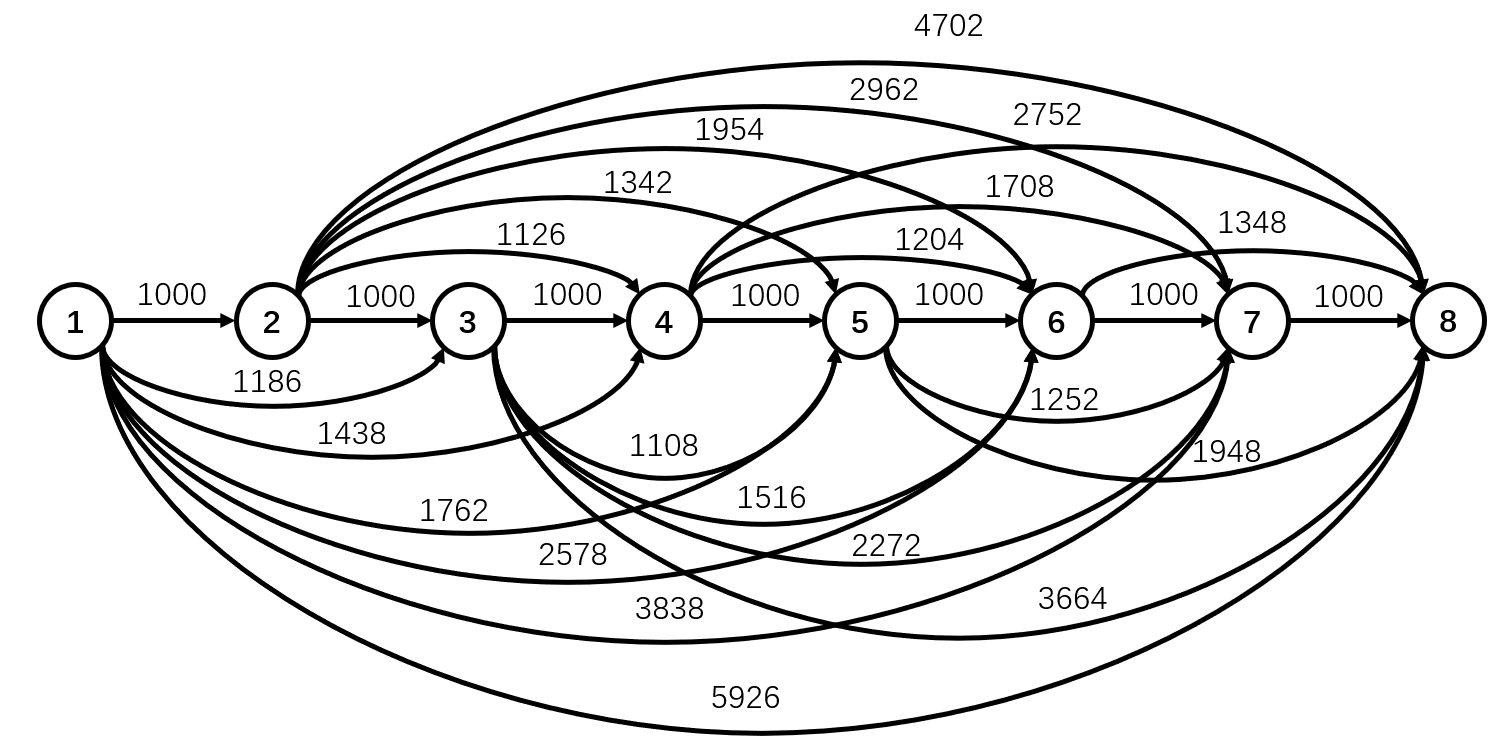
\includegraphics[scale=0.25]{P3b.png}
            \caption{Wagner-Whitin network}
        \end{figure} 
        $\min A[2]=1000,B[2]=\{12\}$
        \\$\min A[3]=\min\{2000,1186\}=1186,B[3]=\{12,13\}$
        \\$\min A[4]=\min\{2186,2126,1438\}=1438,B[4]=\{12,13,14\}$
        \\$\min A[5]=\min\{2438,2294,2342,1762\}=1762,B[5]=\{12,13,14,15\}$
        \\$\min A[6]=\min\{2762,2642,2702,2954,2578\}=2578,B[6]=\{12,13,14,15,16\}$
        \\$\min A[7]=\min\{3762,3014,3146,3458,3962,3838\}=3014,B[7]=\{12,13,14,15,16,57\}$
        \\$\min A[8]=\min\{4762,3629,3710,4190,4850,5702,5926\}=3710,B[7]=\{12,13,14,15,16,57,58\}$
        \begin{figure}[H]
            \centering
            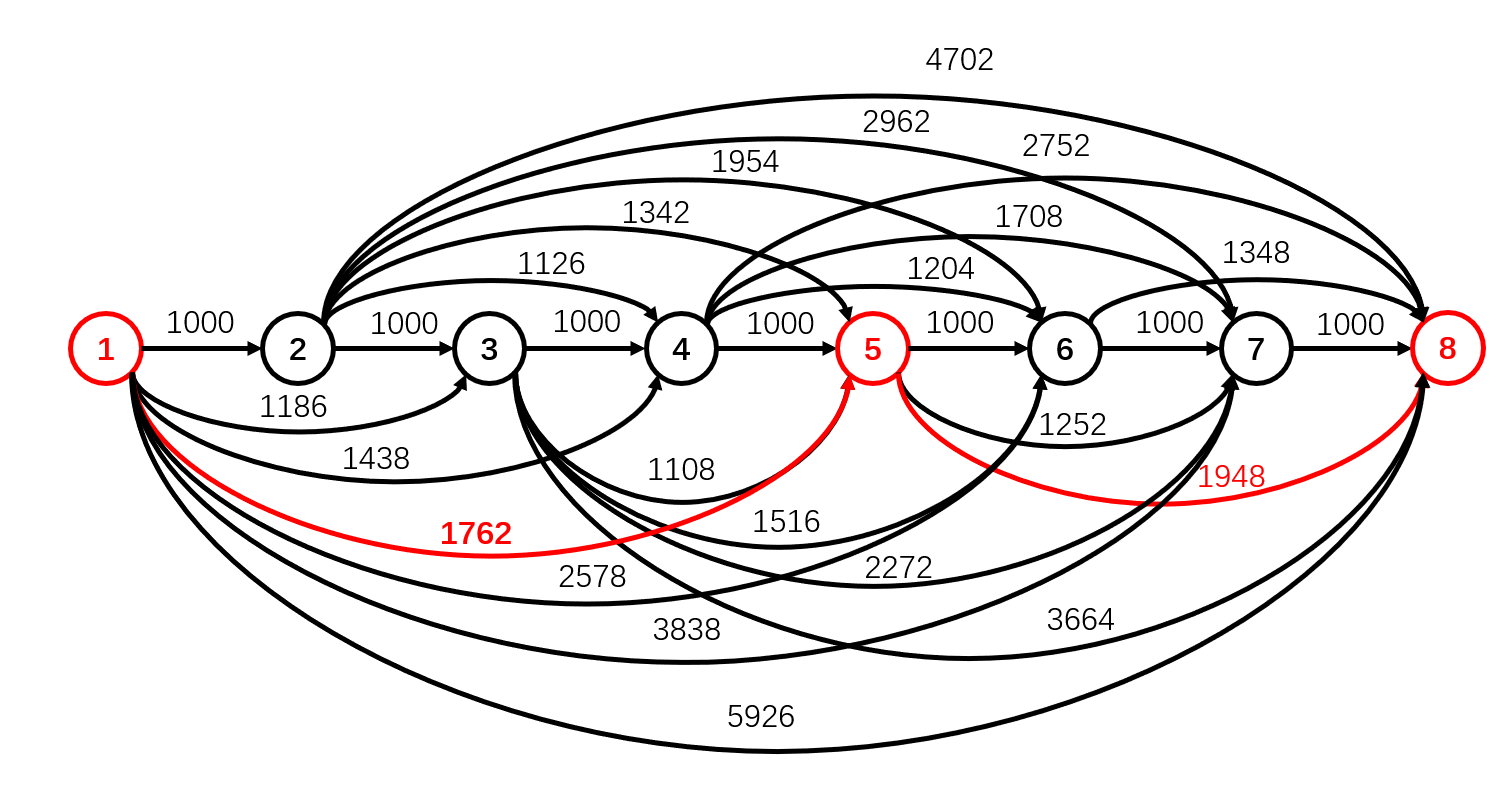
\includegraphics[scale=0.4]{P3b2.png}
            \caption{Wagner-Whitin network}
        \end{figure} 
        Therefore, we should order $d_1,d_2,d_3,d_4$ at Sunday, and order $d_5,d_6,d_7$ at Thursday.
        \\The result is same to dynamic programming with total cost \$3710
        \item The problem is equal to :
        $$\min \qquad \sum_{t=1}^7(1000y_t+1.2x_t)$$
        $$s.t. \qquad x_t=x_{t-1}+q_t-d_t\quad\forall t=1,\cdots,7$$
        $$q_t\leq100000y_t$$
        $$x_t\geq0$$
        $$q_t\geq0$$
        $$y_t\in\{0,1\}$$
        \begin{figure}[H]
            \centering
            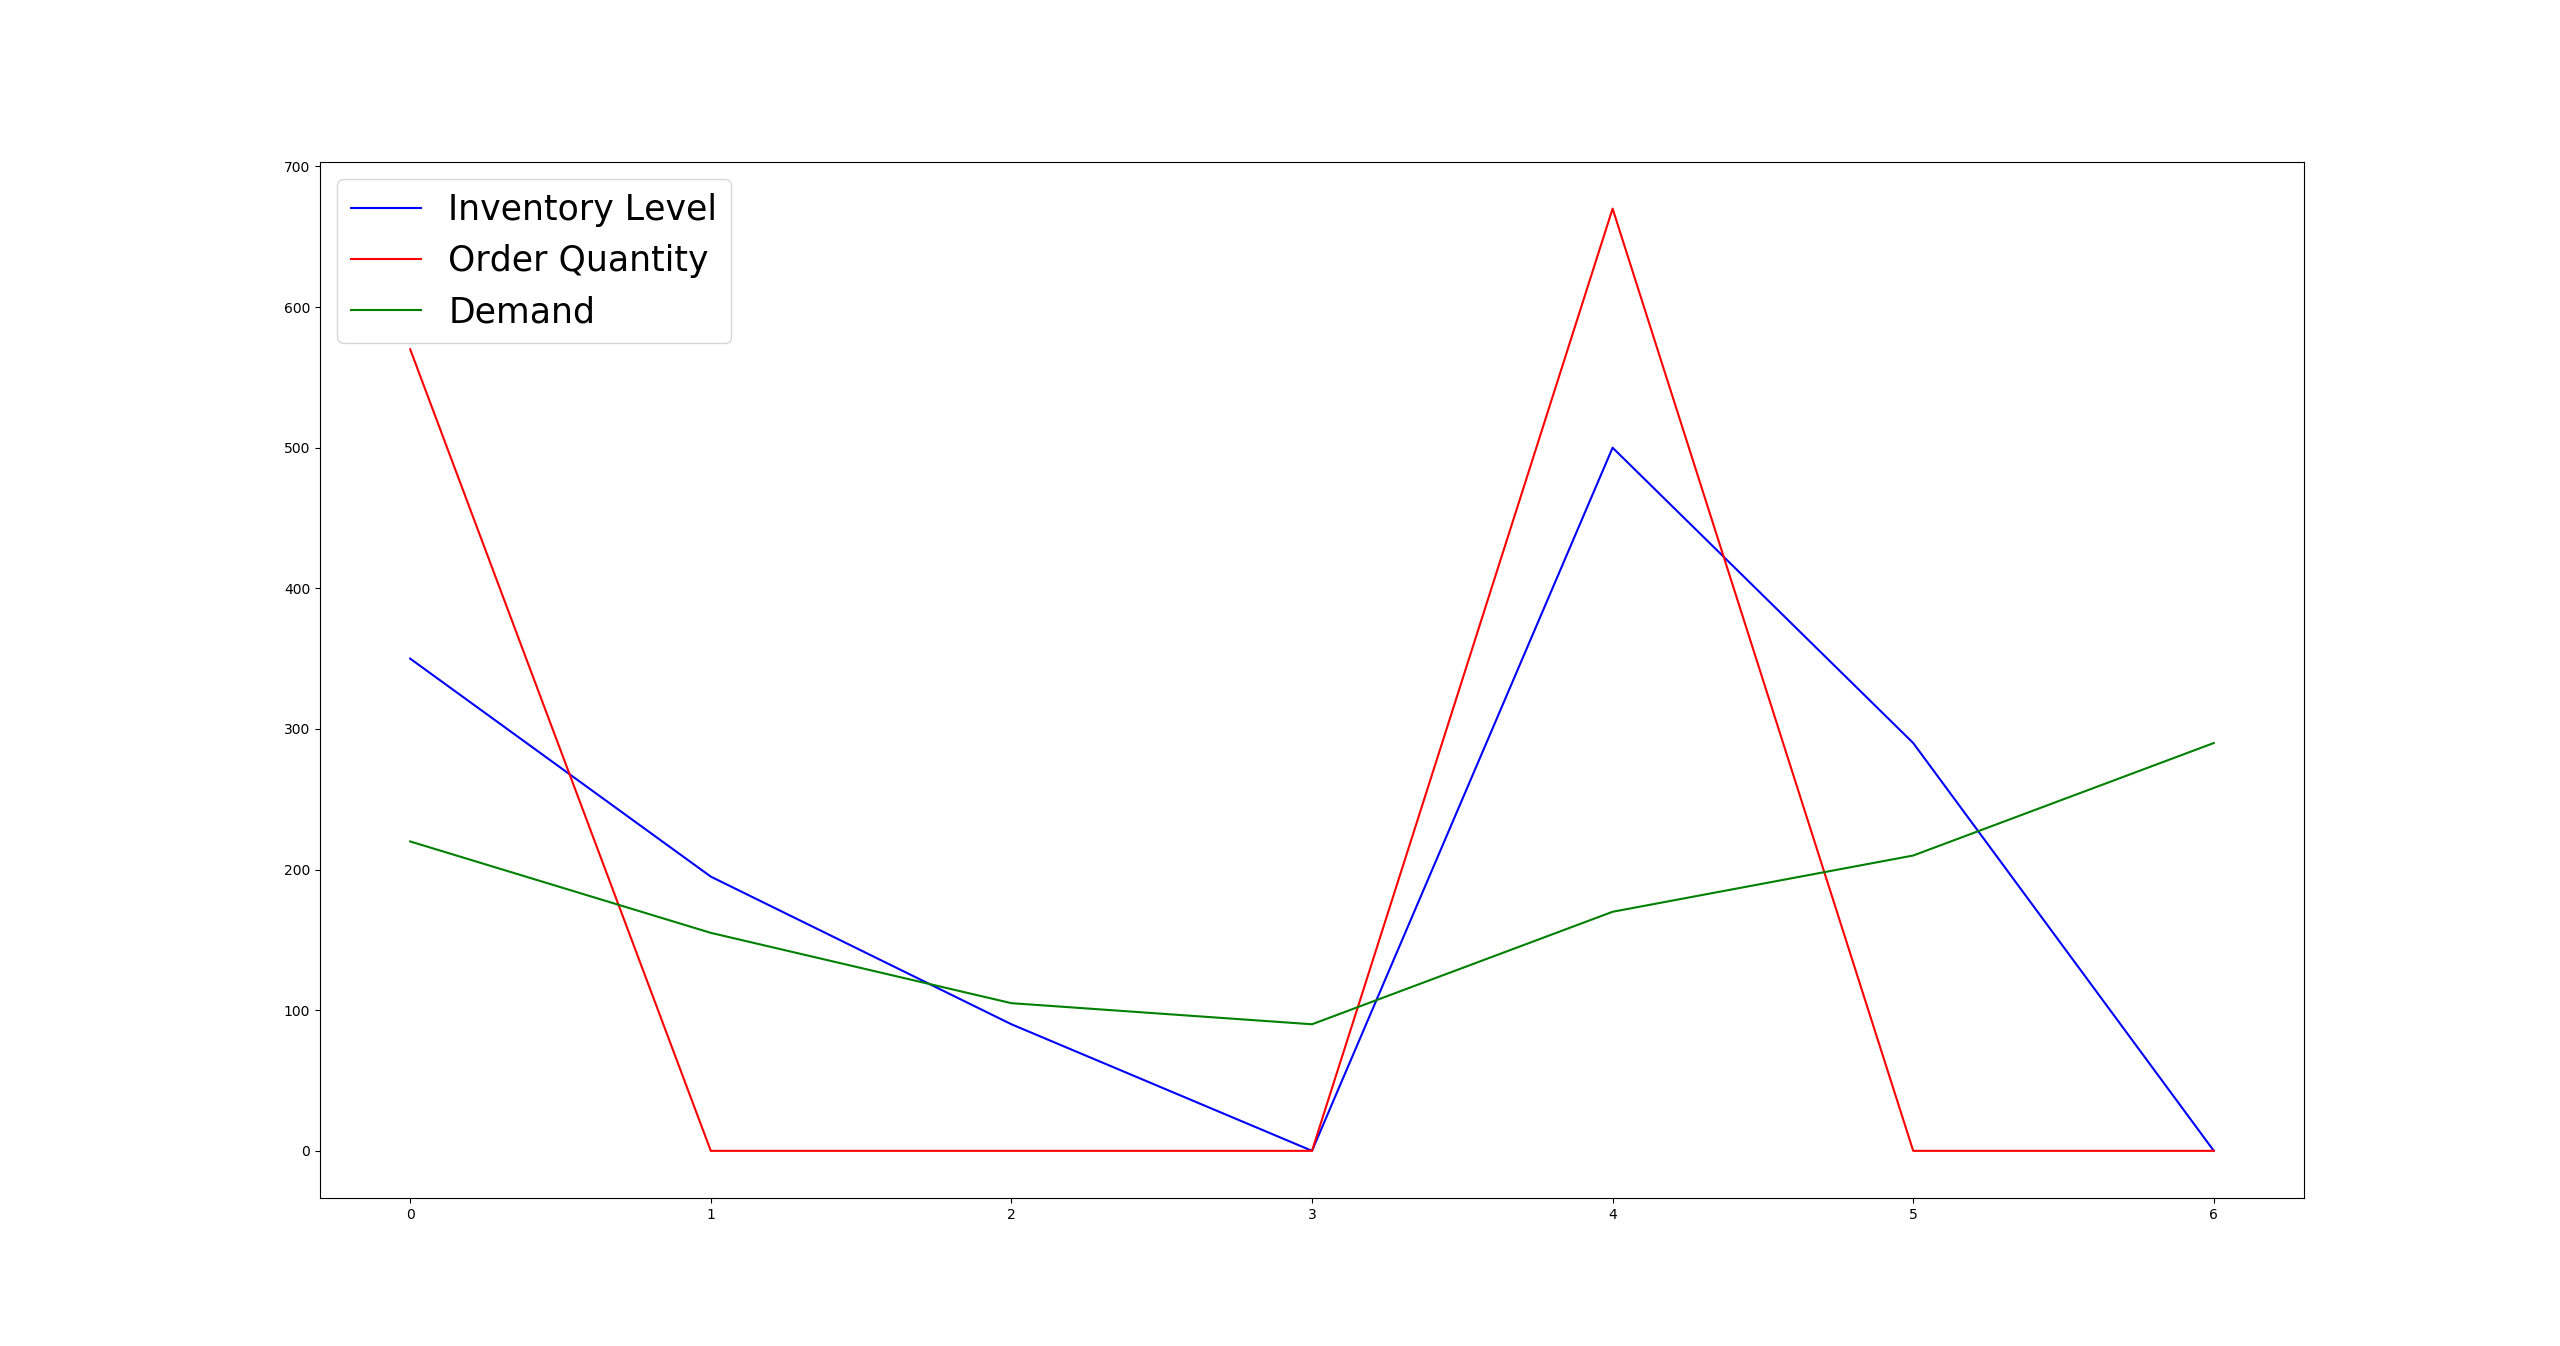
\includegraphics[scale=0.25]{P3c.png}
            \caption{MILP Figure}
        \end{figure} 
        \begin{figure}[H]
            \centering
            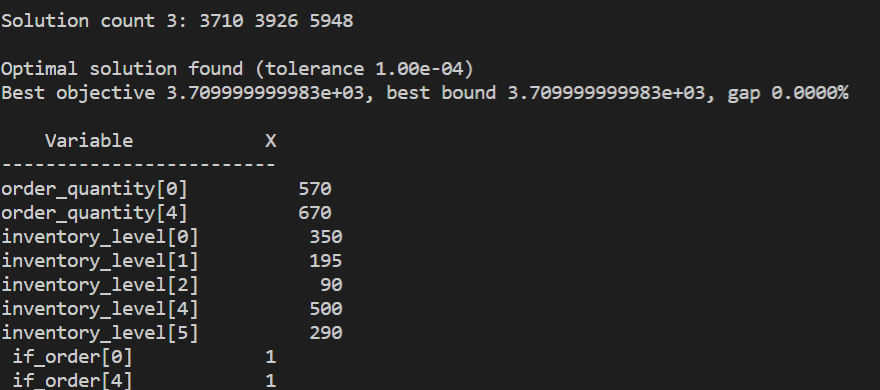
\includegraphics[scale=0.6]{P3c2.png}
            \caption{MILP Result}
        \end{figure} 
        The result shows that we should oder $d_1,d_2,d_3,d_4$ on Sunday, and $d_5,d_6,d_7$ on Thursday.
        \\The optimal cost is \$3710, which is same to last two questions.
    \end{enumerate}
\section{Problem 4}
\begin{enumerate}[(a)]
    \item The duality of the LP problem is:
    $$\min\quad 24y_1+60y_2$$
    s.t. 
    $$3y_1+y_2\geq6$$
    $$2y_1+2y_2\leq14$$
    $$y_1+4y_2=13$$
    $$y_1\geq0$$
    $$y_2\leq0$$
    \item Assume $X=[x_{11},\cdots,x_{1j},x_{21},\cdots,x_{ij}]^T$, where $(i,j)\in E$
    \\For the two constraints, we can let $MX\leq1,NX\leq1$, where $M\in\mathbb{R}^{|I|\times|E|},N\in\mathbb{R}^{|J|\times|E|}$
    \\We can connect $M$ and $N$ together as:
    $ A=\left[\begin{array}{c}   
        M\\ 
        N\\ 
      \end{array}\right]$
      where $A\in\mathbb{R}^{(|I|+|J|)\times|E|}$
    \\Then according to duality and $\textbf{A}^T$, we get $y_i+y_{(|I|+j)}\geq1\quad\forall(i,j)\in E$
    \\Hence the duality of the problem is :
    $$\min\quad \sum_{k=1}^{|I|+|J|}y_k$$
    s.t. 
    $$y_i+y_{(|I|+j)}\geq1\quad\forall(i,j)\in E$$
    $$y_k\geq0\quad\forall k=1,\cdots,|I|+|J|$$
\end{enumerate}
\newpage
\section*{Python Code}
\section*{P1(a)}
    \begin{verbatim}
        import numpy as np
        import pandas as pd
        import matplotlib.pyplot as plt
        df = pd.DataFrame(pd.read_csv(r"D:\PANDA\Study\VG441\Homework\Midterm 1\demands.csv"))
        T=df['time']
        D=df['demands']
        plt.title('Demands against Time')
        plt.scatter(T,D)
        plt.show()
    \end{verbatim}
\section*{P1(b)}
    \begin{verbatim}
        import numpy as np
        import pandas as pd
        import matplotlib.pyplot as plt
        from sklearn import linear_model
        from sklearn.model_selection import train_test_split
        from sklearn.metrics import mean_squared_error, r2_score
        from sklearn.model_selection import cross_val_predict
        df = pd.DataFrame(pd.read_csv(r"D:\PANDA\Study\VG441\Homework\Midterm 1\demands.csv"))
        T=df[['time']]
        D=df[['demands']]
        X_train,X_test,Y_train,Y_test=train_test_split(T, D, test_size=0.8)
        model=linear_model.LinearRegression()
        model.fit(X_train, Y_train)
        model_score = model.score(X_train,Y_train)
        Y_predicted = model.predict(X_test)
        print("Mean squared error: %.2f"% mean_squared_error(Y_test, Y_predicted))
        print('R2 sq: ',r2_score(Y_test, Y_predicted))
        D_predicted = model.predict(T)
        plt.title('Linear Regression Result')
        plt.scatter(T,D_predicted,label='Predicted Demands')
        plt.scatter(T,D,label='Actual Demands')
        plt.legend(loc='upper left', fontsize=25)
        plt.show()
    \end{verbatim}
\section*{P1(c)}
    \begin{verbatim}
        import numpy as np
        import pandas as pd
        import matplotlib.pyplot as plt
        from sklearn import ensemble
        from sklearn.model_selection import train_test_split
        from sklearn.metrics import mean_squared_error, r2_score
        from sklearn.model_selection import cross_val_predict
        df = pd.DataFrame(pd.read_csv(r"D:\PANDA\Study\VG441\Homework\Midterm 1\demands.csv"))
        T=df[['time']]
        D=df[['demands']]
        n=50
        X_train,X_test,Y_train,Y_test=train_test_split(T, D, test_size=0.8)
        params = {'n_estimators': n, 'max_depth': 1, 'learning_rate': 1, 'loss': 'ls'}
        model = ensemble.GradientBoostingRegressor(**params)
        model.fit(X_train, Y_train)
        model_score = model.score(X_train,Y_train)
        Y_predicted = model.predict(X_test)
        print("Mean squared error: %.2f"% mean_squared_error(Y_test, Y_predicted))
        print('R2 sq: ',r2_score(Y_test, Y_predicted))
        D_predicted = model.predict(T)
        title='Gradient Boost Result with n_estimators='+str(n)
        plt.title(title)
        plt.scatter(T,D_predicted,label='Predicted Demands')
        plt.scatter(T,D,label='Actual Demands')
        plt.legend(loc='upper left', fontsize=25)
        plt.show()
    \end{verbatim}
    \section*{P3(c)}
    \begin{verbatim}
        import numpy as np
        import pandas as pd
        from gurobipy import *
        import matplotlib.pyplot as plt
        d = [220, 155, 105, 90, 170, 210, 290]
        T=len(d)
        K, h = 1000, 1.2
        M = 10e5
        # 导入数据
        WW = Model()
        q = WW.addVars(T, lb=np.zeros(T), vtype=GRB.CONTINUOUS, name="order_quantity")
        x = WW.addVars(T, lb=np.zeros(T), vtype=GRB.CONTINUOUS, name="inventory_level")
        y = WW.addVars(T, vtype=GRB.BINARY, name="if_order")
        WW.setObjective(quicksum(K*y[t]+h*x[t] for t in range(T)), GRB.MINIMIZE)
        c1 = WW.addConstrs(q[t] <= M*y[t] for t in range(T))
        c2 = WW.addConstrs(x[t] == x[t-1] + q[t] - d[t] for t in range(1,T))
        c3 = WW.addConstr(x[0] == q[0] - d[0])
        WW.optimize()
        WW.printAttr('X')
        t=np.linspace(0,T-1,T)
        X=[350,195,90,0,500,290,0]
        Q=[570,0,0,0,670,0,0]
        plt.plot(t,X,color='blue',label='Inventory Level')
        plt.plot(t,Q,color='red',label='Order Quantity')
        plt.plot(t,d,color='green',label='Demand')
        plt.legend(loc='upper left', fontsize=25)
        plt.show()
    \end{verbatim}
\end{document}